\documentclass[aps,prb,onecolumn, footinbib, 10pt]{revtex4-2} 


\synctex=1 

%========================= PACKAGES ==================================
\usepackage{dcolumn}
\usepackage{color}
\usepackage{makecell}
\usepackage{tabularx, graphicx}
\usepackage{latexsym}
\usepackage{colortbl}
\usepackage{psfrag}
\usepackage{bbm,bm,array,physics}
\usepackage{dsfont}
\usepackage{float, mathrsfs}

\usepackage{amsmath,amssymb} 
\usepackage{graphicx,comment}

\usepackage[tight]{subfigure} 

\usepackage[dvipsnames]{xcolor} 
\usepackage[papersize={8.5in,11in}]{geometry}
\usepackage[colorlinks=true]{hyperref}
\hypersetup{
    bookmarks=true,         % show bookmarks bar?
    unicode=false,          % non-Latin characters 
    pdftoolbar=true,        % show Acrobat
    pdfmenubar=true,        % show Acrobat 
    pdffitwindow=false,     % window fit to page when opened
    pdfstartview={FitH},    % fits the width of the page to the window
    pdfkeywords={keyword1} {key2} {key3}, % list of keywords
    pdfnewwindow=true,      % links in new window
    colorlinks=true,       % false: boxed links; true: colored links
    linkcolor=magenta, %red,          % color of internal links (change box color with linkbordercolor)
    citecolor=blue,        % color of links to bibliography
    filecolor=magenta,      % color of file links
    urlcolor=blue           % color of external links
} 

\geometry{top=1.5cm, left= 1.5 cm, right= 1.5 cm, bottom= 1.5 cm}        





\def \nn{\nonumber \\}
\def\*#1{\mathbf{#1}} %\bold font
\newcommand{\at}[2][]{#1|_{#2}}


%=======================================================================
\begin{document}
\title{Fermi arcs for generic nodal points hosting monopoles or dipoles}


\author{Ipsita Mandal}
\email{ipsita.mandal@snu.edu.in}

\affiliation{Department of Physics, Shiv Nadar Institution of Eminence (SNIoE), Gautam Buddha Nagar, Uttar Pradesh 201314, India}


\begin{abstract}
%%%%%%%%%%%%%%%%%%%%%
Fermi arcs represent the surface states at the boundary of a three-dimensional topological semimetal with the vacuum, illustrating the notion of bulk-boundary correspondence playing out in real materials. Their special character is tied up with the topological charges carried by the nodes of the semimetal in the momentum space, where two or more bands cross. In fact, they are constrained to begin and end on the perimeters of the projections of the Fermi surfaces of the bands tangentially, signalling their mixing with the bulk states. The number of Fermi arcs grazing onto the tangents of the outermost projection about a given node also reflects the magnitude of the charge at the node (equalling the Berry-curvature monopole), revealing the intrinsic topology of the underlying bandstructure, which can be visualised in experiments like ARPES. Here we take upon the task of unambiguously characterising the analytical structure of these states for generic nodal points, (1) whose degeneracy might be twofold or multifold; and (2) the associated bands might exhibit isotropic or anisotropic, linear- or nonlinear-in-momentum dispersion. Moreover, we also address the question of whether we should get any Fermi arcs at all for topological nodes carrying zero values of monopoles, but representing ideal dipoles.
%%%%%%%%%%%%%%%%%%%%%%%%%%%%%%%%%%%%%%
\end{abstract}

\maketitle

\tableofcontents


%========================= BODY OF THE ARTICLE =========================
\section{Introduction}

Three-dimensional (3d) semimetals harbouring defective points in the Brillouin zone (BZ), where $(2\, \varsigma + 1)$ cross at a nodal-point degeneracy [see Fig.~\ref{figdipole}(a)], provide an intriguing crucible to observe mathematical notions of topology playing out in real-life systems~\cite{burkov11_Weyl,*hosur1, armitage_review, *hosur-review, *yan17_topological, ips-kush-review, bernevig, *bernevig2, grushin-multifold, claudia-multifold}. In the vicinity of a nodal point, the bands form a spin-$\varsigma$ representation of the SU(2) group, being represented as the effective Hamiltonian,
$ \boldsymbol d( \boldsymbol{k} ) \cdot \boldsymbol {S } $, with
$\boldsymbol d( \boldsymbol{k} ) = 
\lbrace d_x ( \boldsymbol{k} ) , d_y ( \boldsymbol{k} ) , d_z ( \boldsymbol{k} )  
 \rbrace.$
%%%%%%%%%%%%%%%%%%%%%
Here, $\mathbf k = \lbrace k_x, \,k_y, \,  k_z  \rbrace$ labels the 3d BZ and $\boldsymbol {S}$ indicates the vector operator comprising the components $ \lbrace S_x, \,S_y, \,  S_z  \rbrace $. Thus, $\boldsymbol {S}$ acts as the well-known angular-momentum operators. The bands are labelled with the eigenvalues of $S_z$, spanning from $- \varsigma $ to $ \varsigma $, which are conventionally referred to as the pseudospin quantum numbers (distinct form the actual spin quantum numbers of the electrons).
%%%%%%%%%%%%%%%%%%%%%%%%%%%%%%
The simplest representative system is an isotropic Weyl node, appearing in semimetals (WSMs)~\cite{burkov11_Weyl, armitage_review, yan17_topological}, carrying $\varsigma = 1/2$ via its two bands. Needless to say, we have now its multifold cousins like the triple-point semimetals (with $\varsigma = 1 $) and Rarita-Schwinger-Weyl (RSW) nodes (with $\varsigma = 3/2$)~\cite{bernevig, long, isobe-fu, tang2017_multiple, ma2021_observation, prb108035428, grushin-multifold, ips-rsw-ph, *ips-shreya,*ips-exact-rsw}. The connection with topology is encoded in the quantum-mechanical phase embodied by the Berry phase, which gives rise to topological vector fields like the Berry curvature (BC) and the intrinsic orbital magnetic moment (OMM) in the momentum space \cite{xiao_review, *sundaram99_wavepacket, *graf-Nband}. In fact, the nodes act as sources/sinks of the flux of the BC-vector field [cf. Fig.~\ref{figdipole}(b)], which explains their singular nature. The magnitude of the BC-monopole carried by a nodal point is synonymous with the Chern number of any closed 2d surface (in momentum space) containing the node inside, giving us the associated topological invariant in terms of the BC-monopole charge. Beyond this simple picture, we are also now aware of more possibilities of the behaviour of the BC where the nodes act as source of higher-order poles \cite{twoband-dipole, graf-hopf, hopf2, *hopf3} (for instance, ideal dipoles, quadrupoles, and so on), thus mimicking our well-known concepts (arising from multipole expansions) of electromagnetism.


Saliently, the existence of the intrinsic topology in the 3d BZ, when treated as a 3d manifold, is reflected in various physical quantities, which can be detected via contemporary experimental techniques. One example is the various types of response that can be detected in transport-measurements, which have been theoretically understood and realised experimentally \cite{timm, ips_rahul_ph_strain, *rahul-jpcm, *ips-ruiz, *ips-tilted, *ips-floquet, ips-kush-review, claudia-multifold, ips-rsw-ph, *ips-shreya}. The list comprises diverse effects such as intrinsic anomalous-Hall effects~\cite{haldane04_berry, goswami13_axionic, burkov14_anomolous}, planar-Hall and Hall coefficients \cite{zhang16_linear, chen16_thermoelectric, nandy_2017_chiral, *nandy18_Berry, amit_magneto,  pal22a_berry, fu22_thermoelectric, timm, staalhammar20_magneto, *yadav23_magneto, ips_rahul_ph_strain, *rahul-jpcm, *ips-ruiz, *ips-tilted, ips-rsw-ph,ips-internode, ips-shreya, ips-spin1-ph,*ips-exact-spin1, ips-nl-ph,  claudia-multifold, ips-exact-kwn}, Magnus-Hall effects~\cite{papaj_magnus, *amit-magnus, *ips-magnus}, circular dichroism \cite{ips-cd1, *ips_cd}, and circular photogalvanic effect \cite{moore18_optical, guo23_light,kozii, *ips_cpge}. However, we must emphasise that perhaps the most unambigous signature comprises the Fermi arcs \cite{yang_Weyl, lv_Weyl_arc, sanchez, spin1-arc,shroter-arc, Yao2020, multifold-rhsi-arc, quad-weyl-arc}, which can be cleanly visualised in experiments like angle-resolved photoemission spectroscopy (ARPES). They represent the surface states in a two-dimensional (2d) surface Brillouin zone (SBZ), always ending tangentially on the boundaries of the projections of the Fermi-surfaces (FSs) of the various bands, where they merge and disappear into the bulk states.


The Fermi arcs are interpreted as the loci of the surface states when we take a surface (say, whose outward normal is along the unit vector, $\boldsymbol{\hat n}$) of a slab consisting of the semimetallic material. In fact, these surface states arise due to the presence of chiral edge modes in 2d slices of the 3d BZ, after we impose open boundary conditions on those slices \cite{burkov11_Weyl, hosur1, hosur-review}. Although we can no longer describe the system in the momentum space for the direction along $\boldsymbol{\hat n}$, the momentum-components perpendicular-to-$\boldsymbol{\hat n}$ (say, $\mathbf k_\parallel$), i.e.,  parallel to the surface itself, remain good quantum numbers (as long as we consider very large spatial dimensions along those directions). Thus, a single (boundary) surface in real space gives us an SBZ, spanned by the components of $\mathbf k_\parallel$, and hosting the Fermi arcs. Although the analytical derivation of surface states, which take the form of Fermi arcs in nodal-point semimetals, is well-understood for the case of Weyl semimetals \cite{witten, hashimoto-arc-weyl, babak-arc-weyl, inti-arc-weyl}, for most other cases, the derivations are system-specific and not generic-enough \cite{witten, okugawa-arc-weyl, liu-arc-mutiweyl, jafari-arc-weyl, trauzettel-arc-weyl, ewelina-surface-states} to be applicable for arbitrary cases of dispersion (for example, anisotropic and/or nonlinear-in-momentum behaviour) and band-crossings. In this paper, our aim is to outline a generic procedure to obtain the analytical forms of the Fermi arcs, which also reflect the Chern numbers of the corresponding 2d slices whose edge states they represent when bulk-boundary correspondence is invoked \cite{burkov11_Weyl, hosur1, hosur-review}.

%%%%%%%%%%%%% fig 0 %%%%%%%%%%%%%%%%%%%%%
\begin{figure}[t]
\centering
\subfigure[]{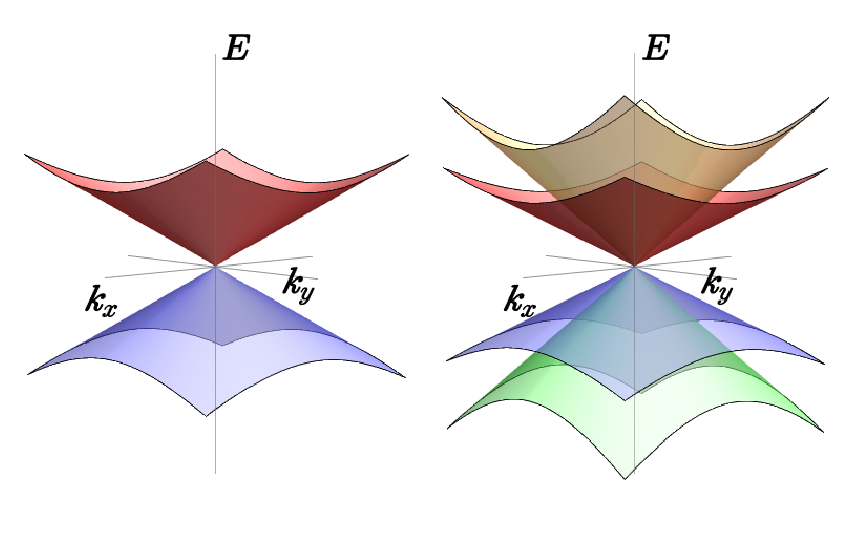
\includegraphics[width=0.35\textwidth]{disp}}\hspace{ 2 cm }
\subfigure[]{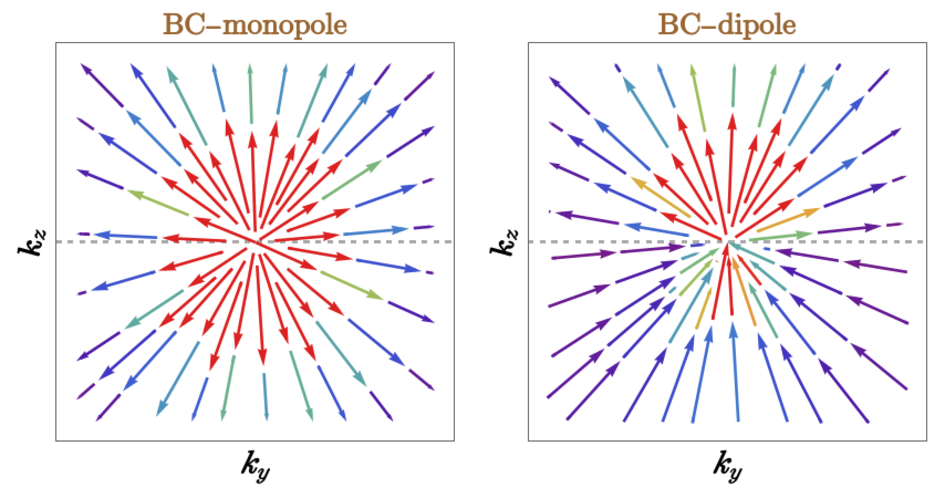
\includegraphics[width=0.45\textwidth]{dipole}}
\caption{(a) Dispersion ($E$) in isotropic twofold (viz. Weyl node) and fourfold (viz. Rarita-Schwinger-Weyl node) band-crossings against the $k_x k_y$-plane. (b) Schematics of BC-flux lines in the $k_x = 0$ planes for a monopole and an ideal dipole. Here, the dipole-axis is orientied along the $k_z$-axis and, hence, the BC goes to zero on the $k_z=0$ plane in the 3d BZ.
\label{figdipole}}
\end{figure}
%%%%%%%%%%%%%%%%%%%%%%

The paper is organised as follows: In Sec.~\ref{secbc}, we lay out our formulation of the boundary conditions, which leads to the solution for the surface states for a generic nodal-point semimetal. Sec.~\ref{secex} is devoted to the application of our method to diverse systems, spanning twofold to multifold ones, linear-in-momentum to quadratic- and cubic-in-momentum ones, and isotropic to anisotropic ones. Furthermore, we also consider two cases where the nodal points represent ideal BC-dipoles rather than monopoles. Finally, we end with a summary and outlook in Sec.~\ref{secsum}.


%%%%%%%%%%%%%%%%%%%%%%%%%%%%%%%%%%%%%%%%%%%
\section{Formulation of boundary conditions}
\label{secbc}

Let us take a single surface at $x=0$ such that the $x<0$ region represent a semi-infinite semimetal, with the bulk Hamiltonian $H(\mathbf k)$, where $\mathbf k \equiv \lbrace k_x, k_y, k_z \rbrace $ and $k =\sqrt{k_x^2 + k_y^2 + k_z^2}$. The translation symmetry is broken along the $x$-axis, and we use the Hamiltonian,
\begin{align}
H_x = H (k_x \rightarrow -i \, \partial_x , k_y, k_z)\,.
\end{align}
Demanding that $H_x $ be Hermitian in the region $x \in [0, \infty)$, we have the physical condition that
\begin{align}
\label{eqherm}
 \int_0^\infty  dx \,\psi^\dagger (x) \, H_x\,\phi (x) = 
 \int_0^\infty  dx\, [H_x\, \psi(x) ]^\dagger\,\phi(x) \,,
\end{align}
%%%%%%%%%%%%%%%%
while considering two bonafide boundary-states, $\psi $ and $\phi$. The current-density operator is defined as
\begin{align}
j_x \equiv \partial_{k_x}  H(\mathbf k) \vert_{k_x \rightarrow -i\, \partial_x}\,.
\end{align}
%%%%%%%%%%%%%%%%
Consequently, Eq.~\eqref{eqherm} also translates into a physically-sensible boundary condition which prohibits the current transmission through the boundary via $ (\psi^\dagger \, j_x \, \psi )\vert_{x=0}= 0$, alternatively known as the hard-wall bc. The boundary modes must behave as decaying wavefunctions of the form of
\begin{align}
\psi (x) = \psi_0 \, e^{- \kappa \, x} \text{ with } \text{Re}(\kappa) > 0\,,
\end{align}
so that the surface states are bound to the boundary at $ x= 0 $. Here, $\psi_0$ is independent of $x$ and any $x$-dependence of $\psi(x)$ is assumed to be contained in the $ e^{- \kappa \, x}$ factor. 



%%%%%%%%%%%%%%%%%%%%%%%%%%%%
\subsection{Witten's formulation for an untilted Weyl node}
\label{secwit}

The effective Hamiltonian in the vicinity of a single Weyl node [cf. Fig.~\ref{figdipole}(a)] is captured by
\begin{align}
\label{eqweyl}
H_W (\mathbf k) = \boldsymbol{\sigma} \cdot {\mathbf k}\,.
\end{align}
Eq.~\eqref{eqherm} translates into
\begin{align}
\label{eqjxweyl}
\psi^\dagger (x)\, \sigma_x \, \phi (x) \vert_{x=0} = 0
\Rightarrow j_x\vert_{x=0} \equiv \psi_0^\dagger\, \sigma_x \, \phi_0  = 0\,.
\end{align}

An energy-independent
boundary condition can be formulated as a local linear restriction on the components of the spinor wave function at the boundary, captured by \cite{witten}
\begin{align}
\label{eqalpha}
\Psi_0 =  M \, \Psi_0\,, \text{ where } M = \cos \alpha \, \sigma_y + \sin  \alpha \, \sigma_z \,.
\end{align}
%%%%%%%%%%%%
This is a good boundary condition because $\sigma_x $ anticommutes with $M$, leading to
\begin{align}
 \psi_0^\dagger\, \sigma_x \, \phi_0 = 
 \frac{1}{2} \left[ \psi_0^\dagger\, \sigma_x \,M\, \phi_0 
 + ( M\, \psi_0)^\dagger\, \sigma_x \, \phi_0 \right ]
  = 0\,.
\end{align}
The variable $\alpha $ acts as a parameter and, by changing $\alpha$, we get Fermi arcs of various shapes and orientations with the restriction that they originate tangentially from the boundary of the projection of the FS on the $k_y k_z$-plane.


%%%%%%%%%%%%%%%%%%%%%%%%%%%%
\subsection{Generic formulation applicable for any kind of nodes}
\label{secgen_method}

For generic nodes with multifold nodes and/or nonlinear powers of the components of $\mathbf k$, Witten's trick will not work, which we will explicitly see why considering some specific examples. Hence, we need an unambigous generic method applicable to derive the equations describing the curves representing the relevant Fermi arcs, which we describe here. Suppose we have an $N$-fold degeneracy at a node, described by the $N \times N $ Hamiltonian, $H_N (\mathbf k)$ in the bulk BZ. Let us look for surface states where the surface-normal is along the direction denoted by the unit vector, $\boldsymbol{\hat n}$, and located at $r_\perp = 0$, where $ r_\perp \equiv \mathbf r \cdot \boldsymbol{\hat n}$. We set our convention that the region $ r_\perp <0 $ represents the region occupied by the semimetallic material, while $r_\perp >0 $ represents the adjoining non-topological region (e.g., vacuum). Dividing up the momentum components along and perpendicular to $\boldsymbol{\hat n}$ as $  k_\perp$ and $\mathbf k_\parallel $, the boundary Hamiltonian is obtained as
\begin{align}
H_{r_\perp} = H_N ( k_\perp\rightarrow -i \, \partial_{r_\perp} , \mathbf k_\parallel)\,.
\end{align}
The imposition of the Hermiticity condition on $H_{r_\perp}$ leads to
\begin{align}
\label{eqherm1}
 \int_0^\infty  dr_\perp \,\psi^\dagger (r_\perp) \, H_{r_\perp}\,\phi (r_\perp) = 
 \int_0^\infty  dr_\perp\, [ H_{r_\perp}\, \psi(r_\perp) ]^\dagger\,\phi(r_\perp) \,,
\end{align}
analogous to Eq.~\eqref{eqherm}. Let us parametrise a solution as
\begin{align}
\psi (r_\perp) = \psi_0 \, e^{- \kappa \, r_\perp} \text{ with } \text{Re}(\kappa) > 0
\text{ and } 
 \psi_0^T  = \begin{bmatrix}
1 & a_1 +i \, b_1 & a_2 + i \, b_2 & \cdots & a_{N-1} + i \, b_{N-1}
\end{bmatrix}.
\end{align}
As argued earlier, (after some manipulations involving integration by parts to convert the integrands into total derivatives) Eq.~\eqref{eqherm1} will turn out to be equivalent to the condition of
%%%%%%%%
\begin{align}
\label{eqcur}
\psi^\dagger  (r_\perp)\, j_{r_\perp} \psi (r_\perp) \big \vert_{r_\perp=0}= 0\,, \text{ where }
 j_{r_\perp} \equiv \partial_{k_\perp}  H_N(k_\perp,  {\mathbf k_\parallel} ) 
\big \vert_{k_\perp \rightarrow -i\, \partial_{r_\perp} }
\end{align}
represents the current-density operator perpendicular to the surface. Next, we need to solve for the eigenvalue equation,
\begin{align}
\label{eqhambdy}
H_{r_\perp} \psi (r_\perp) = E\, \psi (r_\perp)\,,
\end{align}
which leads to $N$ complex-valued equations involving the $(2N+1)$ unknown variables $ E$,
$\kappa_r \equiv \text{Re}(\kappa)$, $\kappa_i \equiv \text{Im}(\kappa)$, $a_1$, $ b_1$, $a_2$, $ b_2$, $\cdots$, $a_{N-1}$,
and $b_{N-1}$. This implies that we have $(2N+1)$ real equations [on including the real equation coming from Eq.~\eqref{eqcur}] at our disposal, which we can use to solve for the same number of unknown variables. In the next section, we will study a variety of systems to see that the above procedure works generically.


%%%%%%%%%%%%%
\section{Specific examples}
\label{secex}

In this section, we will take some specific systems spanning generic features like nonlinear dispersion and multifold band-crossings. In the process, we will also observe how the emergent Fermi arcs reflect the underlying Chern numbers (or, equivalently, monopole charges) of the associated nodes. Additionally, we resolve the issue whether Fermi arcs can appear in nodes harbouring ideal BC-dipoles.

%%%%%%%%%%%%%%%%%%%%%%%%%%%%%%%
\subsection{Untilted nodes of a Weyl semimetal}

%%%%%%%%%%%%% fig 1 %%%%%%%%%%%%%%%%%%%%%
\begin{figure}[t]
\centering
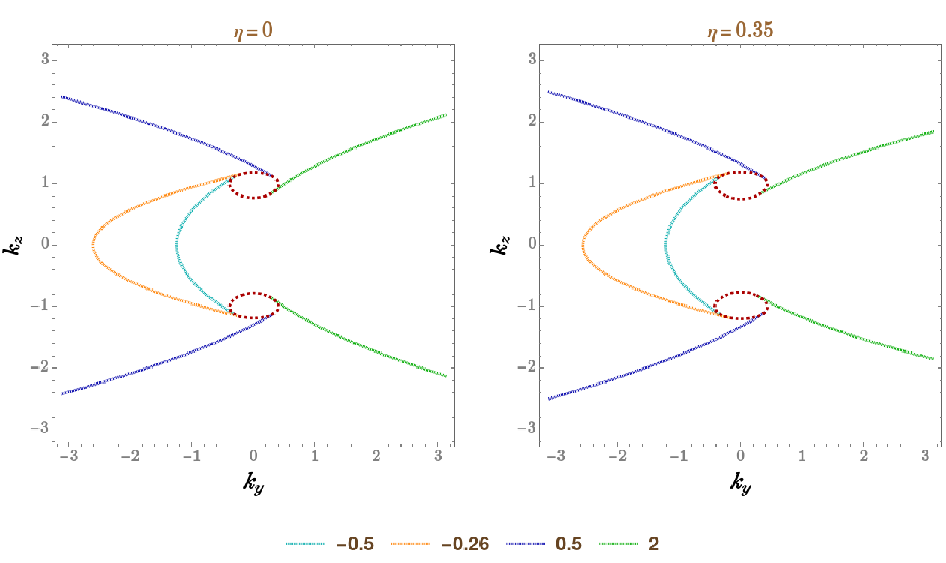
\includegraphics[width=0.75\textwidth]{weylarc}
\caption{A pair of conjugate Weyl nodes: The Fermi arcs represent modes with $E = \mu$, where $\mu =0.5$ and $k_w = 1 $. Each arc corresponds to a distinct value of $b_1$, colour-coded as shown in the plot-legends. The dashed red curves represent the projections of the bulk FSs on the $k_y k_z$-plane.
\label{fig_weyl}}
\end{figure}
%%%%%%%%%%%%%%%%%%%%%%

Let us consider the one-node model given by Eq.~\eqref{eqweyl}, where we want to consider a boundary at $x=0$, indicating $\boldsymbol{\hat n} = \boldsymbol{\hat x} $. Using $ \psi_0^T  = \begin{bmatrix}
1 & a_1 +i \, b_1 \end{bmatrix}$, Eq.~\eqref{eqjxweyl} yields $ a_1  =  0 $. Next, the two components of the matrix equation in Eq.~\eqref{eqhambdy} take the forms of
\begin{align}
& b_1 \left(-i \,\kappa_i+k_y-\kappa_r\right)- E +k_z   = 0 
\text{ and }
-b_1 \left( E + k_z\right)+i \,\kappa_i+k_y+\kappa_r = 0 \nn
%%%%%%%%%%%%%%%%%%%%%%%%%%%%%
\Rightarrow & \, b_1 \left(k_y-\kappa_r\right)- E +k_z = 0\,, \quad 
b_1 \,\kappa_i = 0 \,, \quad \kappa_i = 0 \,, \text{ and }
-b_1 \left(E +k_z\right)+k_y+\kappa_r = 0\,,
\end{align}
%%%%%%%%%%%%%%%%%%%%%
after decomposing them into real and imaginary parts.
We obtain the solutions as $E = \frac{2 \,b_1\, k_y +(1- b_1^2)\, k_z} { 1 + b_1^2 }$, $\kappa_r 
= \frac{\left(b_1^2-1\right) k_y+2 \,b_1\, k_z} { 1 + b_1^2 } $, and $\kappa_i = 0$. We find that $b_1$ plays the role of a parameter, just like $\alpha$ in Eq.~\eqref{eqalpha}. The range of the Fermi arc is determined by the region where $\kappa_r > 0 $, i.e., $ \left(b_1^2-1\right) k_y+2 \,b_1\, k_z > 0$.  The arcs end tangentially on the projections of the bulk FSs, mixing with the bulk states, which is the point where $k_y$ and $k_z$ are as the solutions of the simultaneous equations, $E (k_y, k_z) =\mu$ and $\sqrt{k_y^2 + k_z^2} = \mu$. One can check that at this point, $\lbrace 
k_y, k_z \rbrace = \frac{\mu } { 1+b_1^2 } \lbrace 2\, b_1 , \, 1- b_1^2 \rbrace $ $\Rightarrow \kappa_r = 0 $. Therefore, the surface state ceases to exist at this point, merging with the bulk states.  

For the case of two nodes, separated along the $ k_z$-direction (for example) by an amount $k_w$, we can easily get the nature of the Fermi arcs by the replacement $ k_z \rightarrow (k_z^2 - k_w^2)$. Fig.~\ref{fig_weyl} illustrates the Fermi arcs for four distinct values of $b_1$, when the chemical potential $\mu$ cuts the bandstructure of the surface bands.
%Another intriguing point to note is that, if we set $\mu$ exactly to zero, then the point where $\kappa_r = 0$ represents an \textit{Exceptional Point} (of order two) of the complex matrix $H_x$, where the two eigenvalues and the two eigenvectors coalesce to zero and $ \propto \begin{bmatrix} i \left(b_1^2-1\right) & 2 \, b_1 \end{bmatrix}^T $, respectively.


%%%%%%%%%%%%%%%%%%%%%%%%%%%%%%%
\subsection{Tilted nodes of a Weyl semimetal}

The bulk Hamiltonian in the vicinity of a node, tilted with respect to the $k_x$-axis, is captured by
%%%%%%%%%%%%%%%%%
\begin{align}
\label{eqweylt}
H_W (\mathbf k) = \boldsymbol{\sigma} \cdot {\mathbf k} + \eta\, k_x \, {\mathbb{I}}_{2\times 2}\,.
\end{align}
For this case, on using $ \psi_0^T  = \begin{bmatrix}
1 & a_1 +i \, b_1 \end{bmatrix}$, Eq.~\eqref{eqcur} yields
%%%%%%%%%
\begin{align}
\psi_0^\dagger\, \sigma_x \, \psi_0 + \eta\,\psi_0^\dagger\,  \psi_0 = 0
\Rightarrow  2\, a_1 + \eta  \left( 1+ a_1^2+b_1^2 \right) = 0.
\end{align}
%%%%%%%%%%%%%%%
Next, the two components of the matrix equation shown in Eq.~\eqref{eqhambdy} take the forms of
\begin{align}
&  i \, \kappa_r \left(a_1+i \, b_1+\eta \right)-a_1 \kappa_i-i \,a_1 \,k_y-i \,b_1 \kappa_i
+b_1 \, k_y- E-\eta \, \kappa_i+k_z = 0 \nn
& \text{and }
i \left(i \, \kappa_i + k_y+\kappa_r\right)-\left(a_1+i \, b_1\right) 
\left[ E + \eta  \left(\kappa_i-i \,\kappa_r\right)+k_z\right ] = 0
\nn 
%%%%%%%%%%%%%%%%%%%%%%%%%%%%%
\Rightarrow & \,
-\left(a_1+\eta \right) \kappa_i+b_1 \left(k_y-\kappa_r\right)-E +k_z = 0\,, \quad 
-a_1 \,k_y+\left(a_1+\eta \right) \kappa_r-b_1 \, \kappa_i = 0\,, \nn
& \,-a_1 \left( E +\eta \, \kappa_i+k_z\right)-b_1 \, \eta \, \kappa_r-\kappa_i =0\,, \quad
a_1 \, \eta  \,\kappa_r-b_1 \left( E+\eta \, \kappa_i+k_z\right)+k_y+\kappa_r = 0\,.
\end{align}
%%%%%%%%%%%%
We obtain the solutions as $E =  \frac{b_1 \left [\sqrt{1-\left( 1 + b_1^2 \right)\,
 \eta ^2}+1\right ] k_y+  \left[ \sqrt{1-\left( 1+ b_1^2 \right)\, \eta ^2}  - b_1^2 \right]
 k_z } { 1 + b_1^2} $, 
$\kappa_r  = \frac{\left(b_1^2-1\right) k_y+2 \,b_1\, k_z} { 1 + b_1^2} $, $\kappa_i = 0$, and $a_1 =
\frac{\sqrt{1-\left( 1 + b_1^2\right) \eta ^2} \, -1} {\eta }$.
%%%%%%%%%%%%%%
While for the untilted case (i.e., $\eta = 0$), the projection is the locus of the curve $ k = \mu$ at $k_x = 0$, for the tilted case (i.e., $\eta \neq 0$), it is the locus of the curve $ k = \mu$ at $k_x = -\eta\, \sqrt{ (k_y^2 + k_z^2 ) / (1-\eta^2) }$ (or, equivalently, $k \,\sqrt{1-\eta^2} = \mu $ at $k_x = 0$). This is because, for $\mu \neq 0$, the anisotropic FS (shapeed like a spheroid elongated along the $k_x$-direction) has its largest radius of projection at a negative value of $k_x$. Consequently, the arcs end tangentially on the surface $\sqrt{
(k_y^2 + k_z^2)\,\sqrt{1-\eta^2} } = \mu $. Solving for  $k_y$ and $k_z$ using $E (k_y, k_z) =\mu$ in conjunction, we obtain the coordinates of the Fermi-arc's ending as $\lbrace k_y, k_z \rbrace 
= \frac{\mu} {\left( 1 + b_1^2 \right) \left( 1- \eta ^2\right)}
%%%%%%%%%%%%%%%
\left  \lbrace b_1 \left[ 1 + \sqrt{1-\left( 1+ b_1^2 \right) \eta ^2} \right ], 
 \, \sqrt{1-\left(b_1^2+1\right) \eta ^2} - b_1^2  \right \rbrace $, where of course $\kappa_r $ goes to zero. Again, for the case of two nodes, separated along the $ k_z$-direction (for example) by an amount $k_w$, we can easily get the nature of the Fermi arcs by the replacement $ k_z \rightarrow (k_z^2 - k_w^2)$. Fig.~\ref{fig_weyl} illustrates the Fermi arcs for the two-node case using four distinct values of $b_1$, with $\eta$ set to $0.35$. 


%%%%%%%%%%%%%%%%%%%%%%%%%%
%%%%%%%%%%%%%%%%%%%%%%%%%%%%%%%
\subsection{Triple-point semimetal}


Let us now consider bands carrying pseudospin-1 quantum numbers crossing at threefold-degenerate nodes \cite{bernevig, spin13d1, ips-magnus, grushin-multifold, ips-spin1-ph,*ips-exact-spin1, ips-internode}, representing the so-called triple-point semimetals (TSMs). These are three-band generalisations of the pseudospin-1/2 quasiparticles in Weyl semimetals, with the nodal points acting as Berry-curvature monopoles of magnitude 2. They can be realised in 3d tight-binding models for cold fermionic atoms in cubic optical lattices \cite{cold-atom} and, via \textit{ab initio} simulations, have been identified in materials like TaN, NbN, and WC-type ZrTe \cite{spin13d1, spin13d2, spin13d3, spin13d4}. The effective low-energy continuum Hamiltonian, in the vicinity of a threefold nodal point, is given by
\begin{align}
\label{eqham3d}
\mathcal{H}_{T}(\mathbf  k) = {\mathbf k} \cdot \boldsymbol{\mathcal S}  \,.
\end{align}
Here, $ \boldsymbol{\mathcal S} $ represents the vector spin-1 operator with three components,
\begin{align}
\mathcal{S}_x = \frac {1} {\sqrt{2}}
\begin{bmatrix}
0&1&0\\1&0&1\\0&1&0
\end{bmatrix} ,\quad
\mathcal{S}_y =\frac{1}{\sqrt{2}}
%%%%%%%%%%%
\begin{bmatrix}
0&- i &0\\ \mathrm{i} & 0 &-  i \\
0&  i  &0
\end{bmatrix} ,\quad
%%%%%%%%
\mathcal{S}_z =
\begin{bmatrix}
1&0&0\\0&0&0\\0&0&-1
\end{bmatrix}.
\end{align}
%%%%%%%%%%%%%%%%%%%%%%
The Chern-number values of $\pm 2$ indicate that we must have two distinct Fermi arcs associated with each node \cite{spin1-arc, shroter-arc}. 


%%%%%%%%%%%%% fig TSM %%%%%%%%%%%%%%%%%%%%%
\begin{figure}[t]
\centering
\subfigure[]{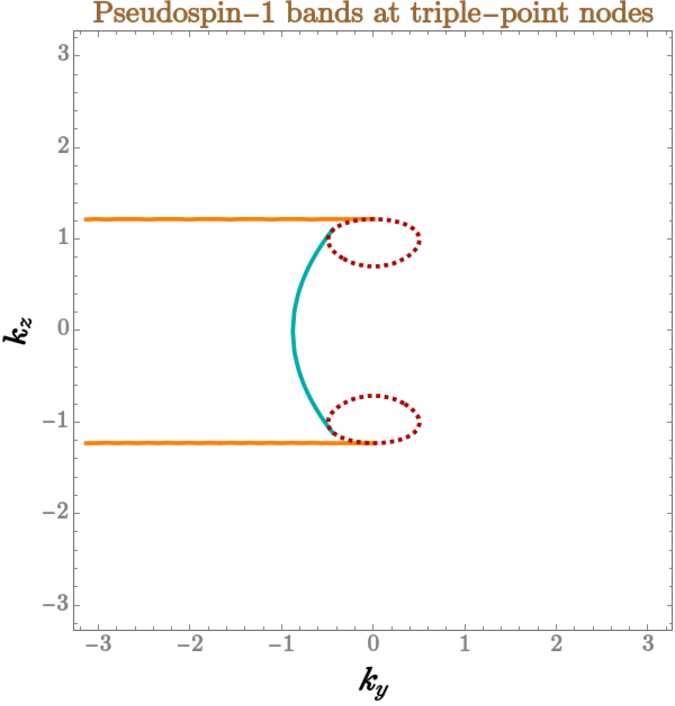
\includegraphics[width=0.36\textwidth]{spin1arc}}\hspace{ 1 cm}
\subfigure[]{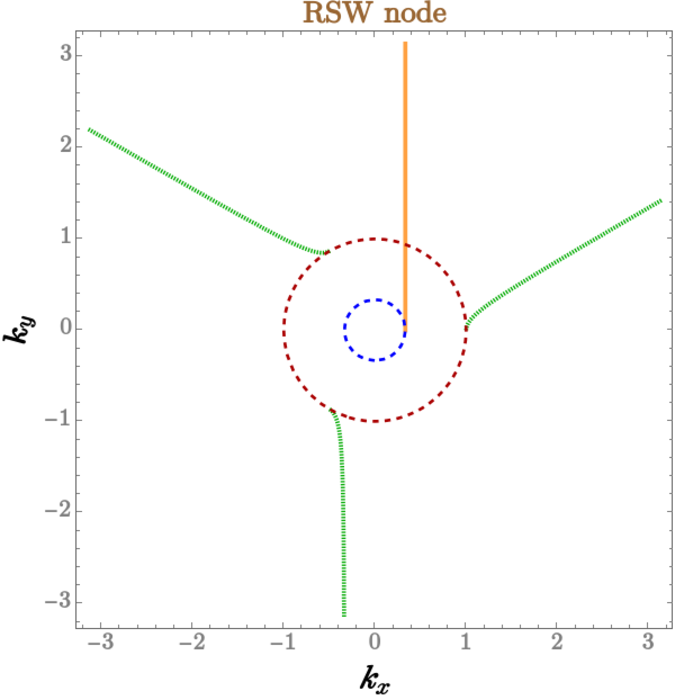
\includegraphics[width=0.365 \textwidth]{RSWarc}}
\caption{(a) A pair of triple-point nodes: The Fermi arcs represent modes with $E = \mu$, where $\mu = 0.5$ and $k_w =1$. The dashed red curves represent the projections of the bulk FSs (of the non-flat bands) on the $k_y k_z$-plane. The two Fermi arcs emanating tangentially from each FS-projection reflect the magnitude Chern number at each node equalling two. The cyan arc has been obtained by setting $b_1 =  -1$.
%%%%%%%%%%%%%%%%%%%%%%%%%
(b) RSW node: Four Fermi arcs emerging from the FS-projections of the two conduction bands, for $\mu=0.5$ and $b_1 = 0$, indicating the Chern number to be four.
\label{fig_spin1}}
\end{figure}
%%%%%%%%%%%%%%%%%%%%%%

Here we note that, although this is a straightforward generalisation of the isotropic Weyl node, we cannot apply Witten's method  (outlined in Sec.~\ref{secwit}) simply because of the fact that $ \mathcal S_x$, $\mathcal S_y$, and $ \mathcal S_z $ \textit{do not anticommute} (unlike the Pauli matrices). For the same reason, the boundary-condition matching procedure of Ref.~\cite{sukhachov-arc-spin1} is inadequate and non-generic for dealing with this system. Hence, our generic method is indispensable 
to explicitly derive the appearances of the Fermi arcs. We use the parametrisation $ \psi_0^T  = \begin{bmatrix}
1 & a_1 +i \, b_1 & a_2 + i\, b_2 \end{bmatrix}$ and consider a boundary at $x=0$. Plugging it in Eq.~\eqref{eqcur} yields
%%%%%%%%% 
\begin{align}
\psi_0^\dagger\, \mathcal S_x\, \psi_0 = 0 \Rightarrow a_1+ a_2 = 0\,.
\end{align}
%%%%%%%%%%%%%%%
Employing the matrix equation, viz. Eq.~\eqref{eqhambdy}, we get
%%%%%%%%%%%%
\begin{align}
&  i \,\kappa_r -\sqrt{2} \left(a_1+i \,b_1\right) \left(E-k_z\right)  = 
\kappa_i+i\, k_y \,,\quad
%%%%%%%%%%%%%%
-\left[ a_1+(1+i) a_2+i \,b_1\right) \left(\kappa_i-i \,\kappa_r\right]
+\left[i \,a_1+(1-i) \,a_2-b_1\right ] k_y
= \sqrt{2} \, E \,, \nn
%%%%%%%%%
& \text{and } \sqrt{2} \, (1+i) \,a_2 \left(E +k_z\right) =
 i \left(i \,\kappa_i+k_y+\kappa_r\right) \nn
 %%%%%%%%%%%%%%%%%
%%%%%%%%%%%%%%%%%%%%% 
& \Rightarrow \,\kappa_i = \sqrt{2} \,a_1 \left(k_z-E\right)\,,\quad
\sqrt{2} \,b_1 \left(k_z- E \right) +  \left(\kappa_r-k_y\right) = 0 \,, \quad
%%%%%%%%%%%%%%%
\left(a_1+a_2\right) \kappa_i+a_2 \left[ \kappa_r-k_y
+ b_1 \left(k_y+\kappa_r\right)\right ] = - \sqrt 2\,E \,, \nn &
%%%%%%%%%%%%%%%%%
\left(a_2+b_1\right) \kappa_i 
= a_2 \left(\kappa_r-k_y\right)+a_1 \left(k_y+\kappa_r\right), \quad
%%%%%
\kappa_i = -\,\sqrt{2}\, a_2  \left( E +k_z\right)\,, \quad
\kappa_r = \sqrt{2} \,a_2 \left( E +k_z\right)+k_y \,.
\end{align}
%%%%%%%%%%%%%
The solutions indeed tell us that there are two Fermi arcs characterised by (1) $E =\frac{2 \sqrt{2}\, b_1\, k_y+4 \,k_z}{ 2 + b_1^2 }-k_z$, $ \kappa_r = \frac{\left(b_1^2-2\right) k_y+2 \sqrt{2} \,b_1\, k_z} { 2 + b_1^2} $, $\kappa_i=0$, $a_1 = 0$, $a_2 = -\, b_1^2/2$, $|b_1 | > 0$, and $b_2 =0$; and (2)  $E = k_z$, $ \kappa_r = -\, k_y $, $\kappa_i=0$, $a_1 = 0$, $a_2 = 0$, $ b_1 = 0$, and $b_2 =0$. For the first arc, $b_1$ plays the role of a parameter and, hence, its shape changes as we vary $b_1$.
%%%%%%%%%%%%%%
The points on the SBZ where $\kappa_r$ goes to zero are found to be $\lbrace k_y, k_z \rbrace =\frac{2\, \mu }{ 2 +b_1^2} \,\lbrace  
 b_1\, \sqrt{2}, \,b_1^2-2\rbrace $ (where $|b_1| > 0$) and $\lbrace k_y, k_z \rbrace = \lbrace  
 0, \,\mu \rbrace $, respectively, for the two Fermi arcs.

For the case of two nodes separated along the $ k_z$-direction (for example) by an amount $k_w$, which is possible when the nodes are not pinned at high-symmetry points for a given crystal structure, we can easily determine the nature of the Fermi arcs by the replacement $ k_z \rightarrow (k_z^2 - k_w^2)$. Fig.~\ref{fig_spin1}(a) illustrates the Fermi arcs for $\mu=0.5$, $k_w =1$, and $b_1=-1$. Since the nodes carry Chern numbers equalling $\pm 2$, we observe two arcs emanating from each FS-projection.


%%%%%%%%%%%%%%%%%%%%%%%%%%%%%%%
\subsection{Rarita-Schwinger-Weyl node in a chiral crystal}

Here we focus on bands carrying pseudospin-3/2 quantum numbers crossing at fourfold-degenerate degenracy-points [cf. Fig.~\ref{figdipole}(a)], widely known as the Rarita-Schwinger-Weyl (RSW) nodes. They appear at the $\Gamma$-points of chiral crystals with appreciable SOC couplings \cite{grushin-multifold, multifold-rhsi, Yao2020, ips-rsw-ph,*ips-shreya,*ips-internode}, hosting a net BC-monopole of magnitude 4. The effective Hamiltonian, in the vicinity of an isotropic RSW node, takes the form of
%%%%%%%%%%%%%%%%%%%%%%%%%%%%%%%
\begin{align}
\mathcal{H}(\boldsymbol{k}) =   {\mathbf k} \cdot \boldsymbol{\mathcal J} \,.
\end{align}
Here, $ \boldsymbol{\mathcal J } = \lbrace {\mathcal J }_x,\, {\mathcal J }_y,\, {\mathcal J }_z \rbrace $ represents the vector operator whose three components comprise the angular-momentum operators in the spin-$3/2$ representation of the SU(2) group. We choose the commonly-used representation with
\begin{align}
{\mathcal J }_x= 
\begin{pmatrix}
	0 & \frac{\sqrt{3}}{2} & 0 & 0 \\
	\frac{\sqrt{3}}{2} & 0 & 1 & 0 \\
	0 & 1 & 0 & \frac{\sqrt{3}}{2} \\
	0 & 0 & \frac{\sqrt{3}}{2} & 0 
\end{pmatrix} , \quad
%%%%%%%%%%
{\mathcal J }_y=
\begin{pmatrix}
	0 & \frac{-i \,  \sqrt{3}}{2}  & 0 & 0 \\
	\frac{i \, \sqrt{3}}{2} & 0 & -i & 0 \\
	0 & i & 0 & \frac{-i \, \sqrt{3}}{2}  \\
	0 & 0 & \frac{i \, \sqrt{3}}{2} & 0 
\end{pmatrix}, \quad
%%%%%%%%%%%%%%%%%%%
{\mathcal J }_z =
\begin{pmatrix}
	\frac{3}{2} & 0 & 0 & 0 \\
	0 & \frac{1}{2} & 0 & 0 \\
	0 & 0 & -\frac{1}{2} & 0 \\
	0 & 0 & 0 & -\frac{3}{2} 
\end{pmatrix}.
\end{align}
%%%%%%%%%%%%%%%%%%%%%%%%
Since the RSW node carries Chern number equalling $ 4 $, we must observe four arcs emanating from the FS-projections of the two nodes being cut by $\mu$. For this case, just for the ease of calculations, we consider a boundary at $z=0$ (just because the $\mathcal J$ matrix has fewer nonzero entries, leading to less cumbersome equations to be solved).
Here again we note that, although this is a fourfold generalisation of the isotropic Weyl node, we cannot apply Witten's method since $ \mathcal J_x$, $\mathcal J_y$, and $ \mathcal J_z $ \textit{do not anticommute} (unlike the Pauli matrices). Hence, we need to utilise our generic method to explicitly derive the equations of the Fermi arcs. We use the parametrisation $ \psi_0^T  = \begin{bmatrix}
1 & a_1 +i \, b_1 & a_2 + i\, b_2 & a_3 + i\, b_3  \end{bmatrix}$ because of the fourfold nature of the bands. Plugging it in Eq.~\eqref{eqcur} yields
%%%%%%%%% 
\begin{align}
\psi_0^\dagger\, \mathcal J_z\, \psi_0 = 0 \Rightarrow 
3 -3\, (a_3^2 + b_3^2)+ a_1^2 +b_1^2 -(a_2^2+b_2^2) = 0\,.
\end{align}
%%%%%%%%%%%%%%%
Employing the matrix equation, viz. Eq.~\eqref{eqhambdy}, we get
%%%%%%%%%%%%%
\begin{align}
& 2\, E =\sqrt{3} \left(a_1+i \,b_1\right) \left(k_x-i \,k_y\right)
-3\, \kappa_i+3\, i \,\kappa_r\,,
%%%%%%%%%%%
\nn & \left(a_1+i \,b_1\right) \left(2 \, E +\kappa_i-i\, \kappa_r\right)
= \left(2 \,a_2+2 \, i \,b_2+\sqrt{3}\right) k_x
+\left( 2\, b_2-2 \,i \,a_2 +i \,\sqrt{3}\right) k_y\,,\nn
%%%%%%%%%%%
& \left(a_2 + i \,b_2\right) \left(2 \,E-\kappa_i + i \,\kappa_r\right)
=\sqrt{3}\, a_3 \left(k_x-i \,k_y\right)
+2\, a_1 \left(k_x+i \, k_y\right) + 2\, i \,b_1 k_x
+i\, \sqrt{3} \,b_3\, k_x - 2 \,b_1\, k_y+\sqrt{3}\, b_3 \,k_y\,, \nn
%%%%%%%%%%%
& \sqrt{3} \left(a_2+i \,b_2\right) \left(k_x + i \,k_y\right)
 = \left(a_3 + i\, b_3\right) \left(2 \, E- 3\, \kappa_i+3 \,i \,\kappa_r\right)
 %%%%%%%%%%%%%%%%%
\nn & \Rightarrow 
2 \, E = \sqrt{3} \, a_1 \,k_x+\sqrt{3} \,b_1 \,k_y-3 \,\kappa_i \,,\quad
\sqrt{3}\, a_1 \,k_y = \sqrt{3} \,b_1 \,k_x + 3 \,\kappa _r \,,\quad
a_1 \left(2 \, E + \kappa _i\right) = \left(2 \,a_2+\sqrt{3}\right) k_x
+2\, b_2 \,k_y-b_1\, \kappa _r  \,,\nn
%%%%%%%%%%%%
& \qquad 2 \, a_2\, k_y = a_1 \,\kappa _r-b_1 \left(2 \, E + \kappa _i\right)
+2\, b_2 \,k_x+\sqrt{3} \,k_y \,,\quad
2 \, b_1\,  k_y = a_2 \left(\kappa _i-2 \,  E \right)+2 \, a_1 \, k_x+\sqrt{3} \, a_3 \, k_x
+\sqrt{3} \, b_3 \, k_y+b_2 \, \kappa _r \,,\nn
%%%%%%%%%%%%%
& \qquad a_2  \,\kappa _r = 2  \,a_1 \, k_y-\sqrt{3}  \,a_3  \,k_y
+b_2 \left(\kappa _i-2  \, E \right)+2  \,b_1 \, k_x+\sqrt{3} \, b_3  \,k_x\,,\quad
2  \,a_3  \,E = 3  \,a_3 \, \kappa _i+\sqrt{3}  \,a_2  \,k_x-\sqrt{3}  \,b_2  \,k_y
+3  \,b_3  \,\kappa _r \,,\nn
%%%%%%%%%%%%
& \qquad 2  \,b_3 \, E = \sqrt{3} \, a_2  \,k_y-3  \,a_3  \,\kappa _r
+3 \, b_3  \,\kappa _i+\sqrt{3}  \,b_2 \, k_x\,.
\end{align}
%%%%%%%%%%%%%%%%%%%%%%
The explicit solutions are long and cumbersome and can be parametrised in terms of one free parameter (which could be any of the $\lbrace a_1, \, a_2, \, a_3, \,b_1, \, b_2, \,b_3 \rbrace $). Hence, we do not write those explicitly. Instead, we show the arcs in Fig.~\ref{fig_spin1}(b) for one single case by setting $\mu=0.5$. The figure shows four Fermi arcs, in total, emanating outside the projection of the outer FS.


%Let us define $k_\parallel   =  \sqrt{k_x^2 + k_y^2}$. We enumerate the results below:
%\begin{enumerate}
%
% %%%%%%%%%%%%%%%%%%%%%%%%%%%%%%%%%%%%%%%%%%%%%%%%
%\item For $ a_1 = 0$:
%\\We get four admissible solutions given by
%\begin{align}
%& E = -\,\frac{3 \,k_y}{2} \,, \quad
%\kappa_r = k_x \,, \quad b_1 = -\sqrt{3} \,, \quad
%a_2 = -\sqrt{3} \,, \quad b_2= 0\,, \quad a_3= 0\,, b_3 = 1\,; \nn
%%%%%%%%%%%%%%%%%%%
%& E = \frac{3 \,k_y}{2} \,, \quad \kappa_r = -\,k_x  \,, \quad
%b_1 = \sqrt{3} \,, \quad a_2 = -\sqrt{3} \,, \quad b_2= 0 \,, \quad a_3= 0\,, \quad b_3= -1 \,;\nn
%%%%%%%%%%%%%%%%%%
%%%%%%%%%%%%%%%%%%%%%%%%%%%%%
%& E = -\,\frac{3 \,k_y \,k_\parallel}{2 \,\sqrt{ k_x^2+ 9\, k_y^2} }
%%%
%\,, \quad \kappa_r = \frac{k_x \,k_\parallel} {\sqrt{ k_x^2+ 9\, k_y^2}}
%%%%%%%%
%\,, \quad b_1 = - k_\parallel  \, \sqrt{\frac{3}{k_x^2+9 \,  k_y^2}}
%%%%
%\,, \quad a_2 =  -\frac{\sqrt{3} \left(6  \, k_x^2  \, k_y^2+k_x^4-3 \,k_y^4\right)}
%{k_\parallel^2 \left(k_x^2+9  \, k_y^2\right)}
%%%%%%%%
%\,, \nn & b_2 = -\frac{8 \,  \sqrt{3}  \, k_x  \, k_y^3}{10 \,  k_x^2  \, k_y^2+k_x^4+9  \, k_y^4}   
%%%%%%%
%\,, \quad  a_3 = - \frac{8  \, k_x  \, k_y^3}{k_\parallel^3 \sqrt{k_x^2+9  \, k_y^2}}
%%%%%%%%
%\,, \quad b_3 = \frac{6  \, k_x^2 \,  k_y^2+k_x^4-3  \, k_y^4}{ k_\parallel^3 \sqrt{k_x^2+9  \, k_y^2}}
%\,;\nn
%%%%%%%%%%%%%%%%%%%%%%%%%%%
%%%%%%%%%%%%%%%%%%
%& E =\frac{3 \,k_y \,k_\parallel}{2 \,\sqrt{ k_x^2+ 9\, k_y^2} }
%%%
%\,, \quad \kappa_r =  -\, \frac{k_x \,k_\parallel} {\sqrt{ k_x^2+ 9\, k_y^2}}
%%%%%%%%
%\,, \quad b_1 = k_\parallel\, \sqrt{\frac{3}{k_x^2+9 \,  k_y^2}}
%%%%
%\,, \quad a_2 =  -\frac{\sqrt{3} \left(6  \, k_x^2  \, k_y^2+k_x^4-3\, k_y^4\right)}
%{k_\parallel^2 \left(k_x^2+9  \, k_y^2\right)}
%%%%%%%%
%\,, \nn & b_2 = -\frac{8 \,  \sqrt{3}  \, k_x  \, k_y^3}{10 \,  k_x^2  \, k_y^2+k_x^4+9  \, k_y^4}   
%%%%%%%
%\,, \quad  a_3 = \frac{8  \, k_x  \, k_y^3}{k_\parallel^3 \sqrt{k_x^2+9  \, k_y^2}}
%%%%%%%%
%\,, \quad b_3 = -\frac{6  \, k_x^2 \,  k_y^2+k_x^4-3  \, k_y^4}{ k_\parallel^3 \sqrt{k_x^2+9  \, k_y^2}}
%\,.
%\end{align}
%
%
%
%
%%%%%%%%%%%%%%%%%%%%%%%
%\item For $b_1 = 0$:
%\\We get four admissible solutions given by
%\begin{align}
%& E = -\,\frac{3 \,k_x}{2} \,, \quad
%\kappa_r = -\, k_y \,, \quad a_1 = -\sqrt{3} \,, \quad
%a_2 = \sqrt{3} \,, \quad b_2= 0\,, \quad a_3= -1\,, b_3 = 0\,; \nn
%%%%%%%%%%%%%%%%%%%
%& E = \frac{3 \,k_x}{2} \,, \quad \kappa_r = k_y  \,, \quad
%a_1 = \sqrt{3} \,, \quad a_2 = \sqrt{3} \,, \quad b_2= 0 \,, \quad a_3= 1\,, \quad b_3=0\,;\nn
%%%%%%%%%%%%%%%%%%
%%%%%%%%%%%%%%%%%%%%%%%%%%%%
%& E = -\,\frac{3 \,k_x \, k_\parallel}{2 \, \sqrt{9\, k_x^2+k_y^2}}
%%%
%\,, \quad \kappa_r = -\, \frac{k_y \,k_\parallel} {\sqrt{9 \, k_x^2+k_y^2}}
%%%%%%%%
%\,, \quad a_1 = -\frac{\sqrt{3} \,  k_\parallel} {\sqrt{9 \,k_x^2+k_y^2}}
%%%%
%\,, \quad a_2 = \frac{\sqrt{3} \left(6 \,k_x^2\, k_y^2-3\, k_x^4+k_y^4\right)}{ k_\parallel^2 
%   \left(9 \,k_x^2+k_y^2\right)}
%%%%%%%%
%\,, \nn & b_2 = -\frac{8\, \sqrt{3}\, k_x^3\, k_y}{10\, k_x^2 \,k_y^2+9 \,k_x^4+k_y^4}
%%%%%%%
%\,, \quad  a_3 = \frac{-6 \,k_x^2 \,k_y^2+3\,  k_x^4-k_y^4}{k_\parallel^{3/2} \sqrt{9 \,k_x^2+k_y^2}}
%%%%%%%%
%\,, \quad b_3 = \frac{8 \,k_x^3 \,k_y}{k_\parallel^{3/2} \sqrt{9 \,k_x^2+k_y^2}}\,;\nn
%%%%%%%%%%%%%%%%%%%%%%%%%%%
%%%%%%%%%%%%%%%%%%
%& E = \frac{3 \,k_x \, k_\parallel}{2 \sqrt{9\, k_x^2+k_y^2}}
%%%
%\,, \quad \kappa_r = \frac{k_y \, k_\parallel}{\sqrt{9 \, k_x^2+k_y^2}}
%%%%%%%%
%\,, \quad a_1 = \frac{\sqrt{3} \,  k_\parallel}{\sqrt{9 \,k_x^2+k_y^2}}
%%%%
%\,, \quad a_2 = \frac{\sqrt{3} \left(6 \, k_x^2\, k_y^2-3\, k_x^4+k_y^4\right)}{ k_\parallel^2 
%   \left(9 \,k_x^2+k_y^2\right)}
%%%%%%%%
%\,, \nn & b_2 = -\frac{8\, \sqrt{3}\, k_x^3 \,  k_y} {10\, k_x^2 \,k_y^2+9 \,k_x^4+k_y^4}
%%%%%%%
%\,, \quad  a_3 = -\,\frac{-6 \,k_x^2 \,k_y^2+3\,  k_x^4-k_y^4}
%{k_\parallel^{3/2} \sqrt{9 \,k_x^2+k_y^2}}
%%%%%%%%
%\,, \quad b_3 = -\,\frac{8 \,k_x^3 \,k_y}{k_\parallel^{3/2} \sqrt{9 \,k_x^2+k_y^2}}\,.
%\end{align}
%
%\item For $a_2 = 0$, we do not get any admissible solutions.
%
%
%%%%%%%%%%%%%%%%%%%%%%%%%%%%%%%%%
%\item For $b_2 = 0$:
%\\We get four admissible solutions given by
%\begin{align}
%& E = -\, \frac{3 \, k_y}{2} \,, \quad \kappa_r = k_x\,, \quad
%a_1 = 0\,,\quad b_1 = -\sqrt 3\,,\quad a_2 = -\sqrt 3 \,,\quad
%a_3 = 0\,,\quad b_3 =1 \,; \nn
%%%%%%%%%%%%%%%%%%%%%
%& E = \frac{3 \, k_y}{2} \,, \quad \kappa_r = -\,k_x\,, \quad
%a_1 = 0\,,\quad b_1 = \sqrt 3\,,a_2 = -\sqrt 3 \,,\quad
%\quad a_3 = 0\,,\quad b_3 = - 1 \,; \nn
%%%%%%%%%%%%%%%%%%%%%
%& E = -\, \frac{3 \, k_x}{2} \,, \quad \kappa_r = -\,k_y \,, \quad
%a_1 = -\sqrt 3 \,,\quad b_1 = 0\,,\quad a_2 = \sqrt 3 \,,\quad
%a_3 = -1 \,,\quad b_3 = 0 \,; \nn
%%%%%%%%%%%%%%%%%%%%%
%& E =  \frac{3 \, k_x}{2} \,, \quad \kappa_r = k_y \,, \quad
%a_1 = \sqrt 3 \,,\quad b_1 = 0\,,\quad a_2 = \sqrt 3 \,,\quad
%a_3 = 1 \,,\quad b_3 = 0 \,.
%\end{align}
%
%\item For $a_3 = 0$, we do not get any admissible solutions.
%
%%%%%%%%%%%%%%%%%%%%%%%%%%%%%%%%%
%\item For $b_3 = 0$:
%\\We get four admissible solutions given by
%\begin{align}
%& E = -\, \frac{3 \, k_x}{2} \,, \quad \kappa_r = -\, k_y \,, \quad
%a_1 =  -\sqrt 3 \,,\quad b_1 = 0\,,\quad a_2 = \sqrt 3 \,,\quad
%b_2 = 0\,,\quad a_3 = - 1 \,; \nn
%%%%%%%%%%%%%%%%%%%%%
%&  E =  \frac{3 \, k_x}{2} \,, \quad \kappa_r =  k_y \,, \quad
%a_1 =  \sqrt 3 \,,\quad b_1 = 0\,,\quad a_2 = \sqrt 3 \,,\quad
%b_2 = 0\,,\quad a_3 =  1 \,;
%%%%%%%%%%%%%%%%%%%%%%%%%%%%%%%%
%\nn & E = -\,\frac{k_x^3-3 \, k_x \, k_y^2 }{2 \, k_\parallel^2} \,,\quad
%%%%%%%%%%%%
%\kappa_r =  k_y-\frac{4\, k_x^2\, k_y}{k_\parallel ^2} \,,\quad
%%%%%%%%%%%%%
%a_1 = -\frac{  6 \,  k_x^2 \, k_y^2 +k_x^4-  3  \,  k_y^4  }{ \sqrt{3} \,k_\parallel^4}\,,\quad
%%%%%%%%%%%%
%b_1 =  \frac{  8 \,  k_x^3 \,  k_y  }{ \sqrt{3} \,k_\parallel^4}\,,\nn
%%%%%%%%%%%%%%%
%& a_2 =  -\frac{  6 \,  k_x^2 \, k_y^2 +k_x^4-  3  \,  k_y^4  }{ \sqrt{3} \,k_\parallel^4}\,,\quad
%%%%%%%%%%%%%%
%b_2 =  -\frac{  8 \,  k_x^3 \,  k_y  }{ \sqrt{3} \,k_\parallel^4} \,\quad
%a_3 =1\,;
%%%%%%%%%%%%%%%%%%%%%%%%%%%%%%%%%%%%%%%%%%%%%%%%
%%%%%%%%%%%%%%%%%%%%%%%%%%%%%%%%
%\nn & E =\frac{k_x^3-3 \, k_x \, k_y^2 }{2 \, k_\parallel^2} \,,\quad
%%%%%%%%%%%%
%\kappa_r =  -\,k_y +  \frac{4\, k_x^2\, k_y}{k_\parallel ^2}\,\quad
%%%%%%%%%%%%%
%a_1 = \frac{  6 \,  k_x^2 \, k_y^2 + k_x^4-  3  \,  k_y^4  }{ \sqrt{3} \,k_\parallel^4}\,,\quad
%%%%%%%%%%%%
%b_1 =  -\frac{  8 \,  k_x^3 \,  k_y  }{ \sqrt{3} \,k_\parallel^4}\,,\nn
%%%%%%%%%%%%%%%
%& a_2 =  -\frac{  6 \,  k_x^2 \, k_y^2 +k_x^4-  3  \,  k_y^4  }{ \sqrt{3} \,k_\parallel^4}\,,\quad
%%%%%%%%%%%%%%
%b_2 =  -\frac{  8 \,  k_x^3 \,  k_y  }{ \sqrt{3} \,k_\parallel^4} \,,
%\quad a_3 =-1\,.
%\end{align}
%
%
%\end{enumerate}




%%%%%%%%%%%%%%%%%%
\subsection{Double-Weyl semimetal}

%%%%%%%%%%%%% fig muti-Weyl %%%%%%%%%%%%%%%%%%%%%
\begin{figure}[t]
\centering
\subfigure[]{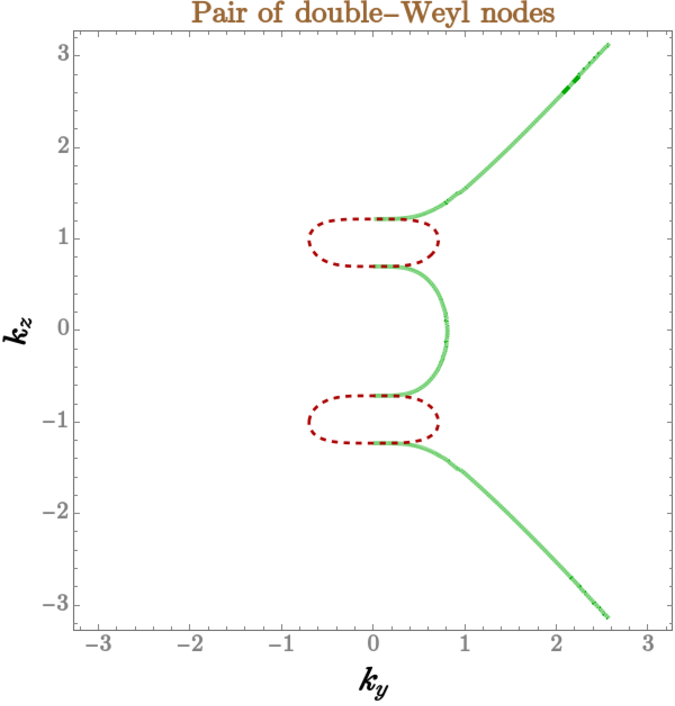
\includegraphics[width=0.36\textwidth]{doubleWeylarc}}\hspace{ 1 cm}
\subfigure[]{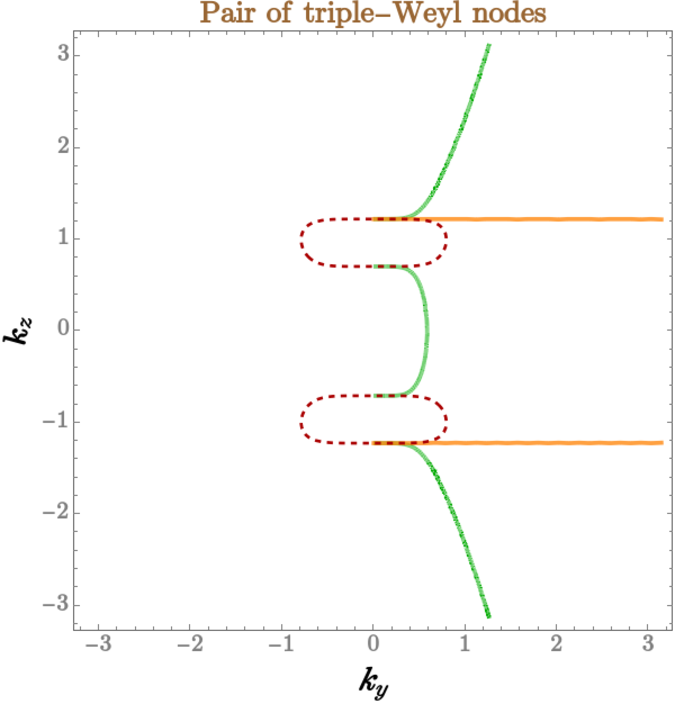
\includegraphics[width=0.36 \textwidth]{tripleWeylarc}}
\caption{The Fermi arcs represent modes with $E = \mu$, where $\mu = 0.5$ and $k_w =1$. (a) A pair of double-Weyl nodes sources two arcs from the perimeter of each FS- projection. Here, $ t = \pi/6$ and $s=1$.
%%%%%%%%%%%%%%%%%%%%%%%%%
(b) A pair of triple-Weyl nodes sources three arcs from the perimeter of each FS-projection. Here, $ t = 0 $ and $s=1$.
\label{fig_multiweyl}}
\end{figure}
%%%%%%%%%%%%%%%%%%%%%%

Double-Weyl nodes can be found in materials like $\mathrm{HgCr_2Se_4}$~\cite{Gang2011} and $\mathrm{SrSi_2}$~\cite{hasan_mweyl16, singh18_tunable}), which exhibits a hybrid of linear dispersion (chosen to be the $k_z$-axis) and quadratic dispersion (in the $k_x k_y$-plane). In the vicinity of such a nodal point, the low-energy effective continuum Hamiltonian is given by \cite{bernevig,bernevig2, fu22_thermoelectric, ips_rahul_ph_strain, ips-ruiz, ips-tilted, chen16_thermoelectric}
\begin{align}
\label{eqhamdw}
H_{dW} = \boldsymbol{d} \cdot \boldsymbol{\sigma}  \,, \text{ where }
\boldsymbol{d} \equiv \left\{ d_x,\, d_y, \, d_z \right\} = \left\{
\frac{k_x^2-k_y^2} {k_0} , \, \frac{2 \,k_x \,k_y} {k_0} ,\, k_z\right\} ,
\end{align}
%%%%%%%%%%%%
where $k_0$ is a material-dependent parameter. For simplicity, we assume the momenta to be scaled such that $k_0$ can be set to 1.
Plugging in the parametrisation of $ \psi_0^T  = \begin{bmatrix}
1 & a_1 +i \, b_1 \end{bmatrix}$ in Eq.~\eqref{eqcur} leads to
\begin{align}
\kappa_i \,\psi_0^\dagger\, \sigma_x \, \psi_0 
=k_y \, \psi_0^\dagger\, \sigma_y \, \psi_0 \Rightarrow
 \kappa_i = \frac{b_1}{a_1} \,k_y \,.
\end{align}
%%%%%%%%%%%%%%%%%%%%%
Additionally, the two components of the matrix of Eq.~\eqref{eqhambdy} provide us with the following:
\begin{align}
&  E = k_z- \left(a_1+i\, b_1\right) \left(i \,\kappa _i-k_y+\kappa _r \right)^2
%%%%%%%%%%%
 \text{ and }
\left(a_1+i \,b_1\right) \left( E + k_z\right)+\left(i \,\kappa _i+k_y+\kappa _r\right)^2 = 0  \nn
%%%%%%%%%%%%%%%%%%%%%%%%%%%%%
\Rightarrow & \, E = k_z -a_1 \left(-2 \left(p^2+1\right) k_y \kappa _r+\left(p^2+1\right) k_y^2
+\kappa _r^2\right)
\,.
\end{align}
%%%%%%%%%%%%
The solutions are found easily after parametrising $ a_1 = a \cos t$ and $ b_1 = a \sin t$:
$E = \frac{\sqrt{k_z^2 \cos^2  t-4 \,k_y^4 \tan ^2 t }}
{\cos t}$, $ \kappa _r =  \frac{ s \, k_y}{\cos (t)} $, , where
$a = s \, \frac{ k_z \,\cos t-\sqrt{k_z^2 \cos ^2 t-4 \,k_y^4 \tan^2 t} }
{2\, k_y^2 \left( 1 + \frac{1}{\cos t} \right)}$ and $s = \pm 1$.
Thus, $t$ serves an undetermined parameter, producing curves of varying shapes. The points on the SBZ where $\kappa_r$ goes to zero are found to be $\lbrace k_y, k_z \rbrace = \lbrace  0,\, \pm \mu \rbrace $.

For the case of two nodes separated along the $ k_z$-direction by an amount $k_w$, we can easily determine the nature of the Fermi arcs by the replacement $ k_z \rightarrow (k_z^2 - k_w^2)$. Fig.~\ref{fig_multiweyl}(a) illustrates the Fermi arcs for $\mu=0.5$, $k_w =1$, and $ t = \pi/6 $. Since the nodes carry Chern numbers equalling $\pm 2$, we observe two arcs emanating from the perimeter of each FS-projection.

%%%%%%%%%%%%%%%%%%
\subsection{Triple-Weyl semimetal}

Analogous to the double-Weyl nodes, there exist triple-Weyl nodes (in materials like transition-metal monochalcogenides~\cite{liu2017predicted}) from which bands with anisotropic dispersion emerge. The triple-Weyl case comprises a hybrid of linear dispersion (chosen to be the $k_z$-axis) and quadratic dispersion (in the $k_x k_y$-plane). In the vicinity of such a nodal point, the low-energy effective continuum Hamiltonian is given by \cite{bernevig, bernevig2, fu22_thermoelectric, ips_rahul_ph_strain, *rahul-jpcm, ips-ruiz, *ips-tilted}
\begin{align}
\label{eqhamtw}
H_{tW} = \boldsymbol{d} \cdot \boldsymbol{\sigma}  \,, \text{ where }
\boldsymbol{d} \equiv \left\{ d_x,\, d_y, \, d_z \right\}=
 \left\{ \frac{k_x^3-3 \,k_x\, k_y^2} {k_0^2}, \, \frac{3 \,k_x^2 \,k_y-k_y^3} {k_0^2} ,
\, k_z\right\} \,,
\end{align}
%%%%%%%%%%%%
where $k_0$ is a material-dependent parameter. Again, for simplicity, we set $k_0$ to 1.
%%%%%%%%%%%%
Plugging in the parametrisation of $ \psi_0^T  = \begin{bmatrix}
1 & a_1 +i \, b_1 \end{bmatrix}$ in Eq.~\eqref{eqcur} leads to
\begin{align}
\left[ 3  \,k_y^2+\left(\kappa _r-i \,\kappa _i\right)^2
+\left(\kappa _r+i \,\kappa _i\right)^2-\kappa _r^2  - \kappa _i^2\right ]
\psi_0^\dagger\, \sigma_x \, \psi_0 
+ 6 \,\kappa _i k_y\, \psi_0^\dagger\, \sigma_y \, \psi_0= 0
\Rightarrow
a_1 \left( \kappa _r^2-3 \,\kappa _i^2+3 \,k_y^2 \right)+6\, b_1 \kappa _i \,k_y = 0\,.
\end{align}
%%%%%%%%%%%%%%%%%%%%%
Additionally, the two components of the matrix of Eq.~\eqref{eqhambdy} provide us with the following:
\begin{align}
&  E = k_z -\left(a_1+i\, b_1\right) \left(\kappa _i+i \,k_y-i \,\kappa _r\right)^3
%%%%%%%%%%%
 \text{ and }
i\, a_1 \left(e+k_z\right) =  b_1 \left( E +k_z\right)
+\left(i \,\kappa _i+k_y+\kappa _r\right)^3    \nn
%%%%%%%%%%%%%%%%%%%%%%%%%%%%%
\Rightarrow & \, E = k_z -a_1 \, \kappa _i 
\left [\kappa _i^2-3 \left(k_y-\kappa _r\right)^2\right ]
-b_1 \left(k_y-\kappa _r\right)
   \left [\left(k_y-\kappa _r\right)^2-3 \,\kappa _i^2\right ], \quad
%%%%%%%%%%%%
b_1 \left( E +k_z\right)
=\left(k_y+\kappa _r\right) 
\left[ 3 \,\kappa _i^2 -\left(k_y+\kappa _r\right)^2\right ] ,\nn  
%%%%%%%%%%%%%%%%
& \quad a_1 \left(k_y-\kappa _r\right) \left[\left(k_y-\kappa _r\right)^2-3 \,\kappa _i^2\right]
= b_1 \,\kappa _i \left[\kappa_i^2-3 \left(k_y-\kappa _r\right)^2\right ], \quad
%%%%%%%%%%%%%%%%%%%%%%%%%%%%%%   
\kappa _i \left [ 3 \left(k_y+\kappa _r\right)^2-\kappa _i^2\right ]
 =a_1 \left( E+k_z\right).
\end{align}
%%%%%%%%%%%%
Finding exact analytical solutions is cumbersome because of the cubit roots involved. Instead, we parametrise $a_1 = a\cos t$ and $b_1 =\sin t$, and we show below the solutions for $t=0$:
(1) $E = k_z$, $\kappa_r  = \pm \, k_y$, $\kappa_i = 0$, and $a =  0 $;
(2) $ E = \frac{1}{3} \sqrt{9\, k_z^2-\frac{512 \,k_y^6}{3}}$, $\kappa_r = s \,k_y$, $\kappa^2 = 
\tilde s \,\frac{2 \, k_y }{ \sqrt 3}$, and $ a =  s\, \tilde s\,
\frac{3 \,\sqrt{3} \,k_z-\sqrt{27\, k_z^2-512\, k_y^6}}{64\, k_y^3}$, where $(s, \tilde s )= \pm 1$.
The points on the SBZ, where $\kappa_r$ for the three arcs goes to zero, are found to be $\lbrace k_y, k_z \rbrace = \lbrace  0,\, \pm \mu \rbrace $.

For the case of two nodes separated along the $ k_z$-direction by an amount $k_w$, we can easily determine the nature of the Fermi arcs by the replacement $ k_z \rightarrow (k_z^2 - k_w^2)$.
Fig.~\ref{fig_multiweyl}(b) illustrates the Fermi arcs for $\mu=0.5$, $k_w =1$, and $s = 1$ (the value of $\tilde s $ does not matter) for the solution detailed above. Since the nodes carry Chern numbers equalling $\pm 3 $, we observe three arcs emanating from the perimeter of each FS-projection.




\subsection{Berry-dipole in a two-band model}
%%%%%%%%%%%%%%



In a specific two-band model, the low-energy effective Hamiltonian in the vicinity of a single node harbouring a Berry-dipole [cf. Fig.~\ref{figdipole}(b)] is captured by \cite{twoband-dipole}
%%%%%%%%%%%%%%%%%
\begin{align}
\label{eqbcd1}
H_{bd} (k_x, k_y, k_z)= 2\, v\, v_z \, k_z \left( k_x \, \sigma_x  +  k_y \,\sigma_y  \right )
+  \left [ v^2 \left( k_x^2 +k_y^2 \right) - k_z^2 \right ] \sigma_z \,.
\end{align}
%Let us set $v=v_z =1 $ for the sake of simplicity.
Being an ideal dipole, this node carries vanishing BC-monopole charge. As such, one might think that there might be no Fermi arcs emerging on the SBZ. However, it turns out Fermi arcs do arise as surface states (on solving systematically using the generic method outlined in Sec.~\ref{secgen_method}), representing edge states on 2d slices carrying opposite Chern numbers. 


Since this is a two-band model, we again use $ \psi_0^T  = \begin{bmatrix}
1 & a_1 +i \, b_1 \end{bmatrix}$. Plugging it in Eq.~\eqref{eqcur} yields
%%%%%%%%% \[Kappa]i \[Psi]dag . ( sz . \[Psi]) vp^2 + kz \[Psi]dag . (sx . \[Psi]) vp
\begin{align}
v_p^2 \,\kappa_i \,\psi_0^\dagger\, \sigma_z \, \psi_0 
+ v_p\, k_z\, \psi_0^\dagger\, \sigma_x \, \psi_0 = 0
\Rightarrow  2 \,a_1\, k_z- v_p  \left(a_1^2+b_1^2-1\right) \kappa_i = 0.
\end{align}
%%%%%%%%%%%%%%%
%%%%%%%%%%%%%%%
Next, the two components of the matrix of Eq.~\eqref{eqhambdy} take the forms of
\begin{align}
&  E =2 \left(b_1-i \,a_1\right)v_p \,v_z \, k_z 
\left ( k_y-\kappa_r  -\kappa_i \right)
+v_p^2 \left[ k_y^2-\left(\kappa_i+\kappa_r\right)^2 \right ]
-v_z^2 \,k_z^2  \nn
%%%%%%%%%%%
& \text{and }
 \left(a_1+i \,b_1\right) 
 \left [ v_z^2\, k_z^2  -v_p^2  \,k_y^2 + v_p^2  \left(\kappa_i+\kappa_r\right)^2  
 - E \right ]  +2\, i \,k_z\, v_p \,v_z 
\left(k_y+\kappa_r + \kappa_i \right)
= 0  \nn
%%%%%%%%%%%%%%%%%%%%%%%%%%%%%
\Rightarrow & \,
E = -2 \, b_1 \,v_p\, v_z \,k_z\left(\kappa_r+\kappa_i \right)
+2\, b_1 \,v_p\, v_z\,k_y\, k_z-v_p^2 
\left(\kappa_i+\kappa_r\right)^2+ v_p^2 \,k_y^2 -v_z^2  \,k_z^2\,,\quad
%%%%%%%%%%
a_1 \, k_z  \left( \kappa_r + \kappa_i-k_y\right) =0\,,\nn
%%%%%%%%%%%%%%%
& a_1 \left(v_p^2 \left(\kappa_r + \kappa_i \right)^2-v_p^2 \, k_y^2 + v_z^2 \,k_z^2 
- E \right) = 0\,, \quad
%%%%%%%%
b_1 \left[v_p^2 \left(\kappa_r + \kappa_i \right)^2
-v_p^2 \,k_y^2 +  v_z^2 \, k_z^2 - E\right ]
+2 \, v_p \,v_z\, k_z \left( \kappa_r + \kappa_i+k_y \right) = 0\,.
\end{align}
%%%%%%%%%%%%
We obtain the solutions as $E =  \frac{k_z\, v_z}{b_1^2}
 \left[2 \,b_1 \,v_p \, k_y +\left(b_1^2-1\right) k_z \,v_z\right] $, 
$\kappa_r  =  k_y-\frac{k_z v_z}{b_1 v_p} $, $\kappa_i = 0$, and $a_1= 0 $.
%%%%%%%%%%%%%%
The points on the SBZ where $\kappa_r$ goes to zero (and the arc becomes tangential to the projection of the FS) are found to be $\lbrace k_y, k_z \rbrace = \pm \,
\sqrt{\frac{\mu }{ 1 +b_1^2}} \,\lbrace  \frac{1}{v_p} , \, \frac{b_1}{v_z} \rbrace $, denoting antipodal points on a FS-projection. In fact, these tangents are inward and outward to the projection, being proportional to $\pm \lbrace  b_1, -1 \rbrace$. 
This shows that that the two arcs are such that one arc is leaving and another is entering into the bulk states which are located at the two hemispheres of the FS, which yield $\pm 1$ on integrating the BC-flux on their surfaces.

%%%%%%%%%%%%% fig dipole  %%%%%%%%%%%%%%%%%%%%%
\begin{figure}[t!]
\centering
\subfigure[]{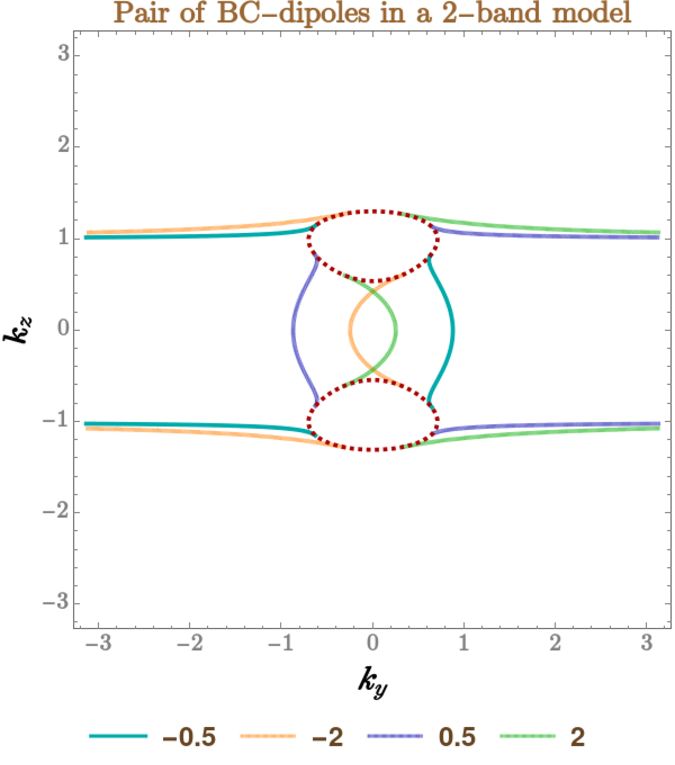
\includegraphics[width=0.36\textwidth]{dipole2bandarc}}\hspace{ 2 cm}
\subfigure[]{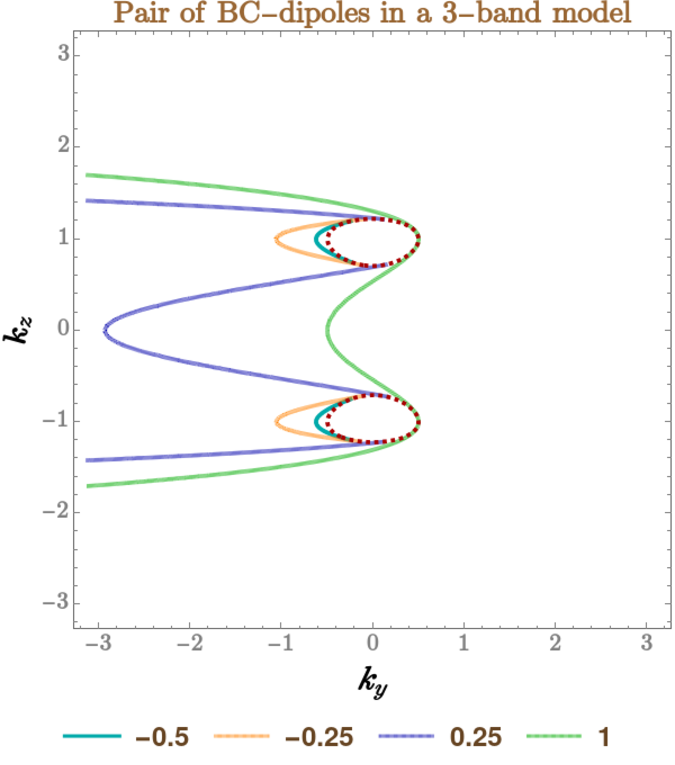
\includegraphics[width=0.36\textwidth]{hopfarc}} 
\caption{The Fermi arcs represent modes with $E = \mu$, where $\mu =0.5$ and $k_w =1$. The dashed red closed contours represent the projections of the bulk FSs on the $k_y k_z$-plane. Each arc corresponds to a distinct value of $b_1$, colour-coded as shown in the plot-legends. A pair of nodes carrying ideal BC-dipoles using the model in (a) Eq.~\eqref{eqbcd1}, with $v_p= v_z=1$; (b) Eq.~\eqref{eqbcd2}. In each case, Fermi arcs graze through each FS-projection at two distinct points, meeting tangentially along a FS-projection.
\label{fig_bcd1}}
\end{figure}
%%%%%%%%%%%%%%%%%%%%%%

If the BZ contains two BC-dipole nodes, separated along the $ k_z$-direction by an amount $k_w$, the answers are obtained by the replacement $ k_z \rightarrow (k_z^2 - k_w^2)$. 
Fig.~\ref{fig_bcd1}(a) shows the resulting Fermi arcs for a particular choice of the parameter-values. Evidently, two Fermi arcs graze past each FS-projection.



%%%%%%%%%%%%%%%%%%%%%%%%%%%%%%%%%%%%%%%%%%%%%%%%%%%%
\subsection{Berry-dipole in a three-band model}
%%%%%%%%%%%%%%

In Ref.~\cite{graf-hopf}, massless multifold Hopf semimetals (MMHSs) have been introduced which host BC-dipoles at nodes where linearly-dispersing bands cross. We consider the simplest case with threefold-degenerate node, captured by the effective continuum Hamiltonian \cite{graf-hopf, hopf2, hopf3},
\begin{align}
\label{eqbcd2}
H_{H} = k_x \,\lambda_1 + k_y \,\lambda_2+ k_z\,\lambda_5\,,
\end{align}
where
\begin{align}
\lambda_1 =  \begin{bmatrix}
 0 & 1 & 0 \\
 1 & 0 & 0 \\
 0 & 0 & 0 \\
\end{bmatrix}, \quad
\lambda_2 = \begin{bmatrix}
 0 & -i & 0 \\
 i & 0 & 0 \\
 0 & 0 & 0 \\
\end{bmatrix}, \quad
\lambda_5 = \begin{bmatrix}
 0 & 0 & -i \\
 0 & 0 & 0 \\
 i & 0 & 0 \\
\end{bmatrix} .
\end{align}
For this 3-band model, we use the parametrisation $ \psi_0^T  = \begin{bmatrix}
1 & a_1 +i \, b_1 & a_2 + i\, b_2 \end{bmatrix}$. For a boundary at $x=0$, plugging it in Eq.~\eqref{eqcur} yields
%%%%%%%%% 
\begin{align}
\psi_0^\dagger\, \lambda_1\, \psi_0 = 0 \Rightarrow a_1 = 0\,.
\end{align}
%%%%%%%%%%%%%%%
Employing the matrix equation, viz. Eq.~\eqref{eqhambdy}, we get
\begin{align}
& \left(b_2-i \,a_2\right) k_z+b_1 \left(-i \kappa_2+k_y-\kappa_r\right) = E 
\text{ and }
 k_y+\kappa_r + i \, \kappa_i = b_1 \, E \nn
 %%%%%%%%%%%%%%%%%
& b_1 \left(k_y-\kappa_r\right)+b_2 \, k_z = E\,,\quad
a_2 \, k_z+b_1 \, \kappa_i = 0\,,\quad \kappa_i = 0 \,, \quad
b_1 \, E =  k_y+\kappa_r\,,\quad a_2\, E = 0\,,\quad b_2\, E = k_z\,.
\end{align}
The solutions turn out to be
$E = \frac{ b_1 \,k_y + \sqrt{b_1^2 \left(k_y^2+k_z^2\right)+k_z^2}} { 1 + b_1^2  }$,
$\kappa_r = \frac{ k_z^2 + b_1 \sqrt{b_1^2 \left(k_y^2+k_z^2\right) }-k_y}{ 1 + b_1^2}$, $\kappa_i  = 0 $,
$a_2 = 0 $, and $b_2  =  \frac{\sqrt{b_1^2 \left(k_y^2+k_z^2\right)+k_z^2}\,-b_1 k_y}{k_z}$. The points on the SBZ where $\kappa_r$ goes to zero (and the arc becomes tangential to the projection of the FS) are found to be $\lbrace k_y, k_z \rbrace = \mu \,\lbrace b_1 , \, \pm\, \sqrt{1-b_1^2}\rbrace $. This also tells us that the parameter $b_1$ is constrained to obey $|b_1|\leq 1 $. 
%%%%%%%%%%%
The corresponding tangents are proportional to $ \lbrace \pm\,\sqrt{1-b_1^2} , \, -b_1\rbrace $ and, hence, are related by flipping the signs of their $k_z$-components, which again leads to the picture that one arc is entering and the other leaving the bulk-states. 
This observation is tied to the fact that these two are associated with the helical edge modes, already observed in experiments \cite{dipole-helical-arc}.

If the BZ contains two BC-dipole nodes, separated along the $ k_z$-direction by an amount $k_w$, the answers are obtained by the replacement $ k_z \rightarrow (k_z^2 - k_w^2)$. 
Fig.~\ref{fig_bcd1}(b) demonstrates the nature of the Fermi arcs for some distinct values of $b_1$. Depending on the value of $b_1$, either two separate Fermi arcs graze past each FS-projection, or the same Fermi arc folds back and rejoins the same FS-projection. 


%%%%%%%%%%%%%%%%%%%%%%%%%%%%%%%%%%%%%%%%%%%%%%%%%%%%
\subsection{Quadruple-Weyl node with monopole-charge 4}
%%%%%%%%%%%%%%


 
A quadruple-Weyl node (QWN) with twofold degeneracy carries BC-monopole charge of magnitude 4 \cite{charge4-1, charge4-2, charge4-3, charge4-4} and can exist only in spinless systems at specific time-reversal symmetric points. Thus, they can appear in electronic bandstructures of materials with
negligible SOC-couplings or in the phonon spectra of artificial crystals (such as photonic crystals), all of which can be treated as spinless systems. Let us take the lattice model of Ref.~\cite{charge4-4}, where two nodes of opposite chiralities emerge at the $\Gamma$- and $R$-points. 
For the node sitting at the $\Gamma$-point can be described by the Hamiltonian,
\begin{align}
\label{eqhamqw}
H_{qW} = \boldsymbol{d} \cdot \boldsymbol{\sigma}  \,, \text{ where }
\boldsymbol{d} \equiv \left\{ d_x,\, d_y, \, d_z \right\}= \left\{\frac{ v \left(k_x^2-k_y^2\right)}{2}, \,\frac{\left(k_x^2+k_y^2-2 \,k_z^2\right)}{2} ,
\,v\, k_x\, k_y\, k_z\right\} .
\end{align}
%%%%%%%%%%%%
Here we fix $v$ to be positive. The energy eigenvalues are given by $\pm \sqrt{ v^2 \left [
2 \,k_x^2 \,k_y^2 \left(2 \,k_z^2-1\right)+k_x^4+k_y^4\right ]
+\left(k_x^2+k_y^2-2\, k_z^2\right)^2 } / 2$. Clearly, the dispersion of the bands is anisotropic, with a cubic dispersion along the $(111)$ direction and quadratic dispersion along any other direction. Here, we expect 4 Fermi arcs to emanate from the nodal point \cite{quad-weyl-arc}, which we will derive explicitly by considering a boundary at $x = 0$.



On using $ \psi_0^T  = \begin{bmatrix}
1 & a_1 +i \, b_1 \end{bmatrix}$, Eq.~\eqref{eqcur} yields
%%%%%%%%% \[Kappa]i (v \[Psi]dag . (sx . \[Psi]) + \[Psi]dag . (sy . \[Psi])) + v ky kz \[Psi]dag . (sz . \[Psi])3]*) 
 %%%%%%%%%%%%%%%%%     
\begin{align}
\kappa_i \left( v\, \psi_0^\dagger\, \sigma_x \, \psi_0 + \psi_0^\dagger\, \sigma_y \, \psi_0 \right)
+ v \, k_y \, k_z \, \psi_0^\dagger\, \sigma_z \, \psi_0 = 0
\Rightarrow  2 \,\kappa_i \left(a_1 \,v+b_1\right) = 
v \left(a_1^2+b_1^2-1\right) k_y \,k_z\,.
\end{align}
%%%%%%%%%%%%%%%
%%%%%%%%%%%%%%%
Employing the matrix equation of Eq.~\eqref{eqhambdy}, we get
\begin{align}
& a_1 \left [ (v-i) \left(\kappa_i-i\, \kappa_r\right)^2- (v+i)\, k_y^2
+2 \,i \,k_z^2\right ]
+b_1 \left[(1+i\,v) \left(\kappa_i-i\, \kappa_r\right)^2
+ (1-i \,v) \,k_y^2-2 \,k_z^2\right ]
=2 \,E +2 \, v \,k_y \,k_z \left(\kappa_i-i\,\kappa_r\right) \nn
 %%%%%%%%%%%%%%%%%
& \text{and } a_1\, E = 
a_1 \,v \,k_y \,k_z \left(\kappa_i-i \,\kappa_r\right)
-i\, b_1 \, E + b_1\, v \,k_y\, k_z \left(\kappa_r+i \,\kappa_i\right)
+\frac{ v+i }{2}  \left(\kappa_i-i\, \kappa_r\right)^2-\frac{(v-i) \,k_y^2}{2} -i \,k_z^2
%%%%%%%%%%%%%%%%%%%%%%
\nn & \Rightarrow
%%%%%%%%%%%%%%
 2\, E + 2\, v \,\kappa_i\, k_y\, k_z
 = b_1 \left(\kappa_i^2+2\, v\,\kappa_i \,\kappa_r + k_y^2-2 \,k_z^2-\kappa_r^2\right)
 -a_1 \left[2 \,\kappa_i \,\kappa_r+v \left(\kappa_r^2-\kappa_i^2\right)+v \,k_y^2\right ],
\nn & 
%%%%%%%%%%%
\qquad a_1 \left(\kappa_i^2+2 \,v\, \kappa_i \,\kappa_r+k_y^2-2 \,k_z^2-\kappa_r^2\right) =
-\,b_1 \left(2 \,\kappa_i\, \kappa_r-v\, \kappa_i^2+v\, k_y^2
+v\, \kappa_r^2\right)+2 \,v \,k_y \,k_z\, \kappa_r\,,\nn & \qquad
%%%%%%%%%%%%%%%%%%%%%%%%%%%%%%%
2\,a_1 \, E =
2  \,a_1  \,v  \,\kappa_i  \,k_y  \,k_z+2  \,\kappa_r 
\left(b_1  \,v  \,k_y \, k_z + \kappa_i\right)+v  \,\kappa_i^2-v \, k_y^2-v \, \kappa_r^2 \,,\nn & \qquad
%%%%%%%%%%%%%%%
2 \,b_1 \, E =
-\,2 \,v\, \kappa_r \left(a_1\, k_y\, k_z+\kappa_i\right)
+2 \,b_1 \,v \,\kappa_i \,k_y\, k_z+\kappa_i^2+k_y^2-2\,k_z^2-\kappa_r^2 \,.
\end{align}
%%%%%%%%%%%%%%
The admissible solutions for $\mu \geq 0 $ are: (1) $E = -\, \frac{v \left(k_y^2-k_z^2\right)}
{\sqrt{ 1 + v^2 }}$,
$\kappa_r = -\,k_y\, k_z$, $\kappa_i = \pm \, 
\sqrt{\frac{ 2 \,k_z^2 - k_y^2 \left[ v^2 \left(k_z^2-1\right) +1\right ]}
{ 1 + v^2}}$, $a_1= \frac{1}{\sqrt{v^2+1}}$, and $b_1  = \frac{-\, v}{\sqrt{v^2+1}}$; and
(2) $E =  \frac{v \left(k_y^2-k_z^2\right)}{\sqrt{ 1 + v^2 }}$,
$\kappa_r = k_y\, k_z$, $\kappa_i = \pm \, 
\sqrt{\frac{ 2 \,k_z^2 - k_y^2 \left[ v^2 \left(k_z^2-1\right) +1\right ]}
{ 1 + v^2}}$, $a_1= \frac{ -\,1}{\sqrt{v^2+1}}$, and $b_1  = \frac{v}{\sqrt{v^2+1}}$.


%%%%%%%%%%%%% fig quad Weyl  %%%%%%%%%%%%%%%%%%%%%
\begin{figure}[t!]
\centering
\subfigure[]{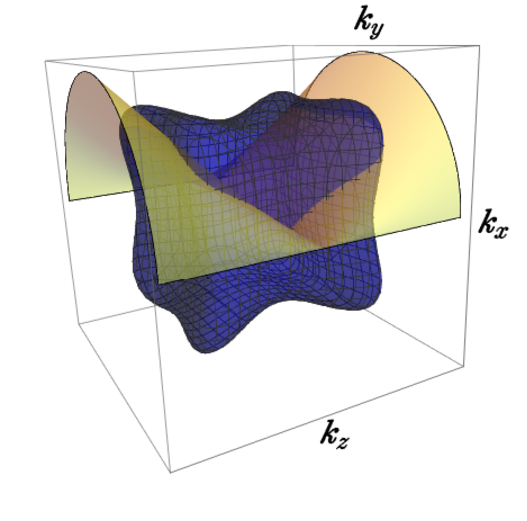
\includegraphics[width=0.3\textwidth]{qWeyl-fs}}\hspace{ 1 cm}
\subfigure[]{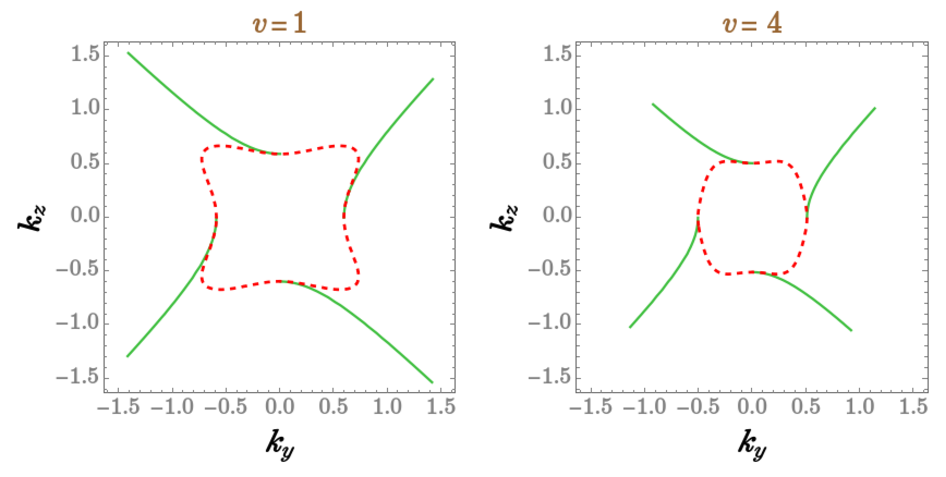
\includegraphics[width=0.6\textwidth]{qweylarc}} 
\caption{(a) The FS-projection is obtained by cutting the 3d FS with the yellow-coloured 2d surface, captured by Eq.~\eqref{figanisofs}. Here, $\mu=0.25$ and $v = 1$. (b) The Fermi arcs represent modes with $E = \mu$, where $\mu =0.25$. The dashed red closed contour represents the projection of the bulk FS on the $k_y k_z$-plane.
\label{fig_qweyl}}
\end{figure}
%%%%%%%%%%%%%%%%%%%%%%


Unlike the cases discussed so far, the projection of the FS on the $x=0$ boundary is not obtained by setting $k_x = 0$. Instead, it is given by the values $k_x = \pm \frac{\sqrt{ 2 \,k_z^2 -2 \,v^2 \,k_y^2\, k_z^2+ (v^2-1)\, k_y^2 }}
{\sqrt{ 1 + v^2 }}$, which leads to the closed curve (lying in the $k_y k_z$-plane) defined by 
\begin{align}
\label{figanisofs}
v\, \sqrt{\frac{ k_z^4- k_y^4 \left(k_z^2-1\right) \left( 1 + v^2 \,k_z^2 \right) + 2 \,k_y^2 \, k_z^2
   \left(k_z^2-1\right)  } { 1 + v^2 } }= \mu \,.
   \end{align}
The case of $v=1$ and $\mu=0.25$ is illustrated in Fig.~\ref{fig_qweyl}(a). Keeping this in mind, the points on the SBZ where $\kappa_r$ goes to zero, becoming tangential to the FS-projection, are found to be $\lbrace k_y, k_z \rbrace = \left\{0, \, \pm \frac{\sqrt{\mu } \,\sqrt[4]{ 1 + v^2}}{\sqrt{v}}\right\}$ and
$\lbrace k_y, k_z \rbrace =
\left\{ \pm \frac{\sqrt{\mu }\, \sqrt[4]{ 1 + v^2}}{\sqrt{v}} , \, 0\right\}$, respectively. Therefore, for different values of, we get Fermi arcs of distinct orientations The tangents to the FS-projection, where the arcs meet the bulk states, are proportional to $ \left \lbrace \pm \,1, \, 0 \right \rbrace $ and $ \left \lbrace  0,\, \pm1 \right \rbrace $. These arcs are thus all leaving the bulk states at the projection.
Fig.~\ref{fig_qweyl}(b) illustrates the arcs for $\mu=0.25$ and two values of $v $. It might seem that the arcs end in thin air, but in actual lattice calculations, they will be found to end on some other nodal point or continue as arcs connecting with those ending on the conjugate QWN-projections located at the $R$-point. The effective Hamiltonian in Eq.~\eqref{eqhamqw}, correct only in the vicinity of the node, of course cannot capture such global details.


\section{Summary and outlook}
\label{secsum}

Our derivations for the nature of surface states in 3d semimetals provide an exhaustive analysis of generic boundary conditions for open boundaries. The main line of argument hinges on the preservation of self-adjointness (i.e., Hermiticity) of the effective Hamiltonian of the corresponding surface, which must host eigenstates that decay exponentially as we move away from the boundary with the topological material. On the side of the material itself, the states must merge with the eigenstates (of the bulk Hamiltonian) representing the 3d bulk states. Through explicit examples, we have shown how the number of Fermi arcs, arising in the SBZ, gives us a clear signature of the net Chern number at a given nodal point, conforming to the well-established notion of bulk-boundary correspondence. However exotic the bandstructure might be, our formalism will work in all generic cases. In the future, we plan to investigate the dynamics of the surface states, for example when a magnetic field is applied, when we can observe quantum oscillations \cite{qtm-osc-ashvin, *hosur-arc-osc}.


% next: Kramers-Weyl node, NLSM, vortex ring SM, Zahid model, type III
% comprehensive analysis of surface states for nodes hosting zero Chern numbers


%%%%%%%%%%%%%%%%
\section*{Acknowledgments}

This research, leading to the results reported, has received funding from the Council of Science \& Technology (CST), U.P.



%%%%%%%%%%%%%%%% bibliography %%%%%%%%%%%%%%%%%%%%%%%%%%%
\bibliography{ref_fa}
\end{document}

Dear Editor,

This is a pioneering work to derive the generic equations which explicitly lead to the expressions for the surface states in a surface Brillouin zone of a 3d Hamiltonian. In this letter, we have used it to characterise Fermi arcs, which are the surface states arising in 3d topological semimetals hosting nodal points. Taking diverse examples, spanning twofold to multifold ones, linear-in-momentum to quadratic- and cubic-in-momentum ones, and isotropic to anisotropic ones, we have demonstrated how the derived states correctly reflect the Chern numbers of the associated nodes. In particular,  we believe that such an analytical study of generic nodes has not been taken upon earlier.

Sincerely,
Ipsita Mandal
%%%%%%%%%%%%%%%%%%%%%%%%%%%%%%%


We model the interface of the semimetal with the vacuum by introducing a mass term as follows
\begin{align}
H_{\mathrm{B}} = \left(k_x^2 - k_\mathrm{W}^2 - \alpha k_{y}^2 + \alpha \partial_z ^2 + M(z) \right)\sigma_x 
+  k_x k_y \sigma_y -i k_x \partial_z \sigma_z,
\end{align}
where $M(z) = 0$ for $z<0$ and $M(z) = M \rightarrow \infty$ for $z>0$. Here we simplify the model by dropping some constants which will be restored later. 

For the localized surface states, we take the ansatz:
\begin{align}
\psi (z)\propto \left\{ 
\begin{array}{cc}
\left( 
\begin{array}{c}
u \\ 
iv%
\end{array}%
\right) e^{\lambda_{<}z}, & z<0 \\ 
\left( 
\begin{array}{c}
u \\ 
iv%
\end{array}%
\right) e^{-\lambda_{>}z}, & z>0%
\end{array}%
\right. ,
\end{align}
where $\mathrm{Re} \lambda_{<}$ and $\mathrm{Re} \lambda_{>}$ are positive. For $z>0$, in the limit of $M \rightarrow \infty$, we have, by taking the ansatz into $H_{\mathrm{B}}\psi = 0$ and neglecting small numbers, 
\begin{align}
\left( M + \alpha \lambda_{>}^2 \right) u -k_x \lambda_{>} v =0 ,
\end{align}
\begin{eqnarray}
\left( M + \alpha \lambda_{>}^2 \right) u -k_x \lambda_{>} v  =0 , \\
\left( M + \alpha \lambda_{>}^2 \right) v -k_x \lambda_{>} u =0 ,
 		\label{model_H_B_surf}      
\end{eqnarray}
leading to 
\begin{align}
k_x \lambda_{>} v  = \pm \left( M + \alpha \lambda_{>}^2 \right) .
\end{align}
Since $\lambda_{>}>0$, we have $u=v$ for $k_x>0$ and $u=-v$ for $k_x<0$. As a result, we have boundaries conditions as
\begin{align}
\psi (z=0)\propto \left( \begin{array}{c} 1 \\ \pm i \end{array} \right) \mathrm{for ~} k_x>0~ (k_x<0).  
\end{align}
With these boundary conditions, we take the ansatz for $z<0$ into $H_{\mathrm{B}}\psi = E\psi$ and we have, for $k_x>0$,
\begin{align}
i\left(k_x^2 - k_\mathrm{W}^2 - \alpha k_{y}^2 + \alpha  \lambda_{<} ^2 \right) + k_x k_y +  i\lambda_{<} k_x =  E.
\end{align} 
Equating the real parts and the imaginary parts separately, we have
$E=k_x k_y$ and 
\begin{align}
\lambda_{<} = \frac{1}{2\alpha} \left\lbrace -k_x  + \sqrt{k_x^2 - 4 \alpha \left(k_x^2 -k_\mathrm{W}^2 - \alpha k_y^2 \right)}\right\rbrace. 
\end{align} 
In order to have  $\mathrm{Re} \lambda_{<}>0$, $k_x$ is limited by
$k_x < \sqrt{k_\mathrm{W}^2 +  \alpha k_y^2 }$. Similarly, for $k_x<0$, we have $E=-k_x k_y$ when $ -\sqrt{k_\mathrm{W}^2 +  \alpha k_y^2 }< k_x$.
In conclusion, when putting back omitted constants, the surface states (the Fermi arcs) survive in $|k_x| <\sqrt{k_\mathrm{W}^2 +  \alpha k_y^2 } $ and take energy 
\begin{align}
E = \frac{v_{\parallel}}{k_\mathrm{W}} |k_x| k_y.
\end{align}
The corresponding wave functions are
\begin{align}
\psi (z<0) = \lambda_{\mathrm{B}} e^{i k_x x} e^{i k_y y} e^{\lambda_{\mathrm{B}} z} \frac{1}{\sqrt{2}}\left( \begin{array}{c} 1 \\ \mathrm{sgn}(k_x) i \end{array} \right), 
\end{align}
where 
\begin{align}
\lambda_{\mathrm{B}} = \frac{m}{\alpha} \left\lbrace - \frac{v_{\parallel}}{k_\mathrm{W}} |k_x|  + \sqrt{ \left(\frac{v_{\parallel}}{k_\mathrm{W}}k_x \right)^2 - \frac{\alpha}{m^2} \left(k_x^2 -k_\mathrm{W}^2 - \alpha k_y^2 \right)}\right\rbrace. 
\end{align} 


%%%%%%%%%%%%%%%%%%%%%%%%%%%%%%%%%%%%%%
\section{Model}



 This leads to \cite{witten, inti, babak}
% PRL127, 056601 (2021)
\begin{align}
0 &= \int_0^\infty dx \left [ \psi^\dagger \, H_x\,\phi - (H_x\, \psi )^\dagger \, \phi 
\right]
\nn & = \int_0^\infty dx \, \partial_x \left[ -2 \, i \, k_z\,\psi^\dagger \, \sigma_x \, \phi
-\partial_x \psi^\dagger \, \sigma_z\, \phi + \psi^\dagger \, \sigma_z\,\partial_x \phi
\right ] \nn
%%%%%%%%%%%%%%%%%%%%
\Rightarrow & \left[  -2 \, i \, k_z\,\psi^\dagger \, \sigma_x \, \phi
-\partial_x \psi^\dagger \, \sigma_z\, \phi + \psi^\dagger \, \sigma_z\,\partial_x \phi
\right ]\vert_{x=0} = 0\,,
\end{align}
since the boundary term at $ x=\infty $ vanishes due to the fact that the wavefunctions must rapidly decay to zero
away from $x=0$. Let us look at the special case when $\phi = \phi = \phi_0 \, e^{-\kappa \, x}$ for $x>0$, with $\phi = \left [
1 \quad v \right]^T $ being independent of $\kappa$, $k_x$, and $ k_y $. This gives us the condition that
\begin{align}
\psi_0^\dagger\, \sigma_z \, \psi = \frac{\text{Im}[\kappa]} {2\, k_z}
\, \psi_0^\dagger\, \sigma_x \, \psi_0 \,.
\end{align}
We note that the expectation value of $\boldsymbol s$ can be generically parametrized as
\begin{align}
\mathbf s \equiv \psi_0^\dagger\, {\boldsymbol \sigma} \, \psi =
\lbrace \sin \alpha \,\cos \beta, \, \sin \alpha \,\sin \beta, \, \cos \alpha \rbrace\,,
\end{align}
Since $\psi_0 $ is assumed to be independent of $\kappa$, $k_x$, and $ k_y $, we get the simple relation that
\begin{align}
\psi_0^\dagger\, \sigma_z \, \psi =  \psi_0^\dagger\, \sigma_x \, \psi_0 = 0\,.
\end{align}
This is captured by $ \mathbf s = \lbrace 0 , \pm 1, \, 0\rbrace $, satisfied by the condition
\begin{align}
\sigma_y \, \psi_0 = \pm \, \psi_0\,.
\end{align}





